%!TEX root = thesis.tex
\chapter{Results}\label{chap:results}
\thispagestyle{plain}

  The following chapter provides all findings from the different experiments detailed in Section~\ref{sec:experimental_setup}. Starting with quantitative results from a single glacier test case, to time series analysis via an ACF and PSD, to a sensitivity analysis of the scaling parameters, and finishing with regional runs for the entire European Alps.

  For all experiments except the sensitivity analysis, the \vas{} is evaluated in comparison to the flowline model. While this gives insights into the drawbacks of simple models and benefits of explicit ice physics, no accuracy assessment can be made without comparison to observational data.

  \section{Single glacier test case} % (fold)
  \label{sec:single_glacier_test_case_results}

    This first test case is intended to get a feel for the \vas{} model and set the stage for the following experiments. The model simulates the evolution of the Hintereisferner (RGI60-11.00897) over 1000 years for three different climate scenarios: an equilibrium climate, and a positive and a negative step change in climate, defined by a temperature bias of \SI{\pm0.5}{\celsius}. Additionally, two different mass balance models are used. The \lstinline`ConstantMassBalance` model simulates a perfectly constant climate and the \lstinline`RandomMassBalance` introduces random year-to-year variability, as the names may suggest. Result are compared to the flowline model. For details about the experimental setup see Section~\ref{sub:single_glacier_test_case_setup}.

    \begin{tldrbox}[Single glacier test case]{tldr:hintereisferner_test_case_results}
      \item Both evolution models produce the same qualitative results, advancing under colder climates and shrinking under warmer climates. The temporal correlation between both models under a random climate is satisfying.
      \item The \vas{} model drastically underestimates changes in glacier geometry compared to the flowline model (up to four times). For example, the relative volume changes for the run with positive mass balance bias amount to $\SI{+17}{\percent}$ for the \vas{} model and $\SI{+71}{\percent}$ for the flowline model. 
      \item The \vas{} does not account for the mass-balance-elevation feedback and therefore produces highly symmetrical results between the positive and negative step change in air temperature. This symmetry can also be seen in the e-folding response times.
      \item The e-folding response times are much shorter for the \vas{} model. For example, the volume response times for the run with positive mass balance bias amount to $\SI{39}{\year}$ for the \vas{} model and $\SI{139}{\year}$ for the flowline model. 
      \item The \vas{} model does not show an asymptotic adjustment but behaves more like a damped harmonic oscillator, whereby the model-internal time scale acts as damping factor.
    \end{tldrbox}

    % overall impression
    The \vas{} model behaves as expected and produces the same qualitative results as the flowline model. The model glacier stays in an approximate equilibrium using the climate around \tstar, and decreases and increases in size for a positive and negative temperature bias of \SI{\pm0.5}{\celsius}, respectively. However, the \vas{} model underestimate changes in geometry compared to the flowline model. This is true for both the constant and random climate scenario, whereby the \lstinline`RandomMassBalance` model, with its year-to-year variations, produces more short term variability (most obviously). Figure~\ref{fig:hintereisferner} shows the time series for ice volume, surface area and glacier length for all climate scenarios and both evolution models.

    % temporal correlation between VAS and flowline
    The modeled glacier advances and retreats forced by the random climate scenarios show a weak but highly significant correlation between the two evolution models (with correlation coefficients $0.34 \leq r \leq 0.58$ and p-values of $p \ll 0.01$). Given that the implementations of the mass balance models are almost identical between the \vas{} model and the flowline model, this is the first indication that the differences must arise from the geometry models. For both models, the ice volume exhibits the highest year-to-year variability, since volume changes happen instantaneously, i.e., over a single time step. The changes in surface area and glacier length are smoother, accounting for the glacier's response time. However, the flowline model shows generally less short term variabilities but stronger long term variabilities than the \vas{} model, indicating longer response times. This assumption is backed by the model behavior under the constant climate scenarios. Qualitatively speaking, the flowline model takes longer to reach a new equilibrium (about 400 years) than the \vas{} model (about 200 years). A quantitative analysis of the response times follows after the evaluation of the equilibrium values. 

    % Equilibrium values
    % ------------------

    % segue and introduction
    For the following discussion about the new equilibrium values, only the constant climate scenarios are considered (if not stated otherwise). It is assumed that the model glacier has reached a new equilibrium 1000 years after the climate perturbation. Hence, the equilibrium values are taken as the final values at year \lstinline`t = 1000`. This assumption seems valid, given that the fluctuation of volume, area and length are in the order of only \SI{0.01}{\percent}\footnotemark{} over the last 200 years of the simulations.
    \footnotetext{The fluctuations are computed as the relative difference between minimum and maximum value during that period. The relative difference between two values $a$ and $b$ refers to their absolute difference relative to the average between them $\left|\frac{a-b}{(a+b)/2}\right|$.}
    Table~\ref{tab:hintereisferner_equilibrium_values} shows all new equilibrium values in response to the positive and negative step changes in climate. Percentage values refer to the normalized glacier geometries to their respective initial values, which facilitates the comparison.
    
    % underestimation
    The most apparent result is that the \vas{} model underestimates all changes in glacier geometry compared to the flowline model. While the \vas{} model estimates a volume change of \SI{+17}{\percent} and \SI{-15}{\percent}, the flowline estimates \SI{+72}{\percent} and \SI{-42}{\percent}, for the negative and positive temperature perturbation, respectively. In other words, the flowline glacier grows more than four times larger and shrinks more than two and a half times smaller than the \vas{} glacier.
    The changes in surface area are slightly less underestimated, with values of \SI{+12}{\percent} and \SI{-11}{\percent} for the \vas{} model and \SI{+33}{\percent} and \SI{-23}{\percent} for the flowline model. The glacier length of the \vas{} model does hardly change at all. The year-to-year changes of glacier length estimated by the \vas{} model range between \SI{-11}{\meter} and \SI{+8}{\meter}, corresponding to a maximal change of \SI{2}{\percent} of the initial values. This results in a total length change of \SI{\pm7}{\percent} for the \vas{} model over the entire simulation, which is roughly five to six times less than the changes of \SI{+44}{\percent} and \SI{-39}{\percent} for the flowline model. The continuous length records for Hintereisferner from 1939 to 2003 \citep{Leclercq2014} show an average yearly absolute length change of $26\pm{}\SI{21}{\meter}$ (mean $\pm$ standard deviation) and a maximum of over \SI{100}{\meter}. That amounts to an maximum observed yearly length changes of \SI{1.6}{\percent} in relation to the glacier length of \SI{6.9}{\kilo\meter} in 2003. It seems that the values of relative length change of the \vas{} are comparable to observations, the absolute values, however, are far too low. This is the another indication that the \vas{} model cannot resolve all the same processes as a dedicated ice physics models can.
    
    % symmetry
    The changes in glacier geometries produces by the \vas{} model are highly symmetrical. Absolute changes ice volume, surface area and glacier length differ by a maximum of \SI{7}{\percent}, \SI{3}{\percent}, and \SI{2}{\percent}, respectively, between the run with positive and negative mass balance perturbation\footnote{The percentages correspond to the relative difference, as explained above}.
    Again, this cannot be explained by the mass balance models. The climate scenarios used for this experiment are all based on an equilibrium climate. If the input climate is not altered by a temperature bias, the model glacier will stay in its equilibrium state under the constant climate scenario. Under a random climate scenario the model glacier will show some year-to-year variability, but still fluctuation around the same equilibrium values. This specific equilibrium mass balance can be approximated as a linear function of temperature bias (with $r^2 > \SI{99.9}{\percent}$), for small enough temperature biases between \SI{-1}{\celsius} and \SI{+1}{\celsius}. Thereby, the slopes of the linear functions and consequentially the initial specific mass balance are almost identical between the \vas{} and flowline model: \SI{+309}{\milli\meter\waterequivalent\per\year} and \SI{-320}{\milli\meter\waterequivalent\per\year} for the \vas{} model and \SI{+307}{\milli\meter\waterequivalent\per\year} and \SI{-323}{\milli\meter\waterequivalent\per\year} for the flowline model. The initial mass balance values are quite symmetrical for both evolution models and can, therefore, not be the cause of the \vas{} model's symmetric equilibrium results.
    However, since this study looks for benefits of a dedicated ice physics model rather than flaws of the \vas{} model, the question should be “What allows the flowline model to produces asymmetric results?”. % the question should not be “What makes the \vas{} model results symmetric?” but much rather
    And the answer is the mass-balance-elevation feedback. The flowline model continuously adjusts the surface elevation of each grid cell and passes the elevation information onto the mass balance model\footnote{Implementation note: the mass balance feedback can be adjusted via the \lstinline`mb_elev_feedback` parameter of the \lstinline`FlowlineModel` class}. Suppressing the mass-balance-elevation feedback for the flowline model run results in a volume change of \SI{+38}{\percent} and \SI{-34}{\percent}. These results are symmetric and lower than with mass-balance-elevation feedback in place. The relative changes in ice volume are reduced to about twice the values produces by the \vas{} model.
    % segue and introduction of next section
    It has been shown, that the responses of the \vas{} model and the flowline model to a step change in climate are qualitatively similar but do not compare quantitatively. While the absolute equilibrium values are still in the same order of magnitude, they differ substantially. But what about the time domain? The following paragraphs look at temporal characteristics of the glacier model's response.

    % Time scales
    % -----------

    % time scales computed by the vas model
    The implementation of the \vas{} model includes the corresponding response time scaling to estimate temporal changes (see Section~\ref{sub:glacier_evolution_model_implementation}). For a proper response time scaling, the length response time scale $\tau_L$ and the area response time scale $\tau_A$ must be estimated. The length response time scale can be estimated as ratio between ice volume and mass turnover \citep{Johannesson1989}, the area response time scale then follows from geometric considerations. The model-internal time scales computed for the Hintereisferner under a constant equilibrium climate amount to $\tau_L \approx \SI{38}{\year}$ and $\tau_L \approx \SI{12.5}{\year}$. Those values are rather low compared to other findings of $\tau_L \approx \SI{100}{\year}$ \citep{Greuell1992, Schuster2020}. However, it is possible that the used time scales are merely model parameters and do not correspond to the typically used e-folding time scales.
    
    % e-folding time scales
    % The flowline model has no inherent measure for a glacier's time scale.
    Processes evolving exponentially to an equilibrium can be characterized by their e-folding response time. The assumption that a glacier's geometry changes exponentially is valid for small enough perturbations in climate. The e-folding response time is computed as the time after which the initial difference between a glacier's geometric property (such as ice volume, surface area or glacier length) and its new equilibrium value has decreased by a factor of $1-\mathrm{e}^{-1}\approx\SI{63}{\percent}$. For comparability, e-folding time scales are computed for both evolution models and all geometric properties. The values can be found in Table~\ref{tab:hintereisferner_time_scales}.
    As was to be expected, volume response times $\tau_V$ are smallest, followed by $\tau_A$ and $\tau_L$. As already qualitatively estimated above, the \vas{} model adjust between two times and six times faster to the temperature perturbation of \SI{\pm0.5}{\celsius} than the flowline model. This is especially visible for the growing glacier, where the flowline model takes almost \SI{120}{\year} longer to reach a new equilibrium than the \vas{} model does ($\tau_{V,\text{fl}}=\SI{142}{\year}$ vs. $\tau_{V,\text{vas}}=\SI{24}{\year}$).
    
    % symmetry
    The results of the \vas{} model are again very symmetric between the positive and negative temperature perturbation. The \vas{} e-folding time scales range within \SI{9}{\percent} of each other, while the flowline response time scales vary up to \SI{55}{\percent}\footnotetext{The percentages correspont to the relative difference, as explained above.}. Suppressing the mass-balance-elevation feedback for the flowline model results in similarly symmetric result.
    % oscillation
    It has to be noted, that the length e-folding response time for the \vas{} model $\tau_{L,\text{vas}}\approx\SI{55}{\year}$ is over twenty years (\SI{\approx 30}{\percent}) longer than the model-internal time scale.
    However, the \vas{} model does not show an asymptotic or exponential adjustment. The adjustment of glacier geometries looks like the signal of an underdamped oscillator, with a strongly discernible overshoot. The damping factor seems to be controlled by the model-internal time scale, which could allow for an additional tuning parameter. A closer look at this oscillatory behavior is provided in Section~\ref{sec:sensitivity_to_model_internal_time_scales_results}

    % scaling for single glacier, sensitivity to scaling constant
    While Hintereisferner is not representative for all Alpine glaciers, the same experiment performed on other single glaciers yields similar results (see Appendix~\ref{appendix_A}). For some glaciers (e.g., Mer de Glace, Glacier d'Argentière) the change in relative ice volume is comparable between the two evolution models. However, this is merely a mathematical artifact, since the initial ice volume estimated by the scaling relation is much smaller than the one from the numerical ice thickness inversion. The absolute values of ice volume and ice volume change are still drastically underestimated by the \vas{} model. Unlike ice volume and glacier length, the initial surface area is equivalent for both models. This generally results in better agreement of estimated final equilibrium areas, even though the glacier areas simulated by the \vas{} model show far more and stronger fluctuations under random climates.
    Anyway, all of those observations are not robust, since scaling relations are developed to work best on a global or at least a regional scale. The scaling constant $c$ is a random variable which can vary drastically from glacier to glacier. It is possible that the global mean value of $c=\SI{0.034}{\kilo\meter^{3-2\gamma}}$ is a bad fit for the characteristics of Hintereisferner (or any other single glacier). A detailed look at the model's sensitivity to the scaling constant is provided in Section~\ref{sec:sensitivity_to_scaling_parameters_results}.

    
    % Table showing the Hintereisferner equilibrium values, geometries as columns including initial values
    \begin{table}[htp]
      \centering
      \small
      \ra{1.4}

      \caption{Hintereisferner (RGI60-11.00897) equilibrium values after 1000 years of model evolution in response to a step change in climate of $\Delta T = $\SI{\pm0.5}{\celsius} relative to the average climate between 1912 and 1942. Percentage values in parenthesis indicate normalized changes in respective to their initial values.}
      \label{tab:hintereisferner_equilibrium_values}
      
      \begin{tabular}{@{}rcrlcrlcrl@{}}
        \toprule
        {} & \phantom{a} & \multicolumn{2}{c}{\textbf{Length [\si{\kilo\meter}]}} & \phantom{a} & \multicolumn{2}{c}{\textbf{Area [\si{\square\kilo\meter}]}} & \phantom{a} & \multicolumn{2}{c}{\textbf{Volume [\si{\cubic\kilo\meter}]}} \\
        \midrule
        \textbf{Initial values} \\
        V/A scaling & \phantom{a} & 4.89 & & \phantom{a} & 8.04 & & \phantom{a} & 0.60 & \\
        Flowline & \phantom{a} &  6.90 & & \phantom{a} & 8.04 & & \phantom{a} & 0.80 & \\
        $\bm{\Delta T}$\textbf{ = \SI{-0.5}{\celsius}} \\
        % \cmidrule{1-10}
        V/A scaling & \phantom{a} & 5.25 & (\SI{+7}{\percent}) & \phantom{a} & 8.98 & (\SI{+12}{\percent}) & \phantom{a} & 0.70 & (\SI{+17}{\percent}) \\
        Flowline & \phantom{a} &  9.80 & (\SI{+42}{\percent}) & \phantom{a} & 10.64 & (\SI{+33}{\percent}) & \phantom{a} &  1.38 & (\SI{+72}{\percent}) \\
        \addlinespace
        $\bm{\Delta T}$\textbf{ = \SI{+0.5}{\celsius}} \\
        % \cmidrule{1-10}
        V/A scaling & \phantom{a} & 4.54 & (\SI{-7}{\percent}) & \phantom{a} & 7.12 & (\SI{-11}{\percent}) & \phantom{a} & 0.50 & (\SI{-15}{\percent}) \\
        Flowline & \phantom{a} &   3.80 & (\SI{-45}{\percent}) & \phantom{a} & 6.16 & (\SI{-23}{\percent}) & \phantom{a} & 0.46 & (\SI{-42}{\percent}) \\
        \bottomrule
      \end{tabular}
    \end{table}

    % Table showing the e-folding time scales for Hintereisferner, time scales as columns
    \begin{table}[htp]
      \centering
      \small
      \ra{1.4}

      \caption{e-folding time scales for Hintereisferner (RGI60-11.00897) in response to a step change in climate of $\Delta T = $\SI{\pm0.5}{\celsius} relative to the average climate between 1912 and 1942. Time scales are computed for changes in ice volume, surface area and glacier length, denoted as $\tau_V$, $\tau_A$ and $\tau_L$, respectively.}
      \label{tab:hintereisferner_time_scales}
      
      \begin{tabular}{@{}rcrcrcr@{}}
        \toprule
        {} & \phantom{a} & $\bm{\tau_L}$ \textbf{[\si{\year}]} & \phantom{a} & $\bm{\tau_A}$ \textbf{[\si{\year}]} & \phantom{a} & $\bm{\tau_V}$ \textbf{[\si{\year}]} \\
        \midrule
        $\bm{\Delta T}$\textbf{ = \SI{-0.5}{\celsius}} \\
        % \cmidrule{1-10}
        V/A scaling & \phantom{a} & 55 & \phantom{a} & 36 & \phantom{a} & 24 \\
        Flowline & \phantom{a} &  184 & \phantom{a} & 160 & \phantom{a} & 142 \\
        \addlinespace
        $\bm{\Delta T}$\textbf{ = \SI{+0.5}{\celsius}} \\
        % \cmidrule{1-10}
        V/A scaling & \phantom{a} & 52 & \phantom{a} & 33 & \phantom{a} & 22 \\
        Flowline & \phantom{a} & 118 & \phantom{a} & 111 & \phantom{a} & 80 \\
        \bottomrule
      \end{tabular}
    \end{table}

    % Figure showing Hintereisferner time series plots - on page
    \begin{figure}[p]
      \centering

      % VAS volume
      \begin{subfigure}[b]{0.476\textwidth}
        \caption{\Vas{} model, relative ice volume}
        \label{fig:hintereisferner:volume_vas}
        \centering
        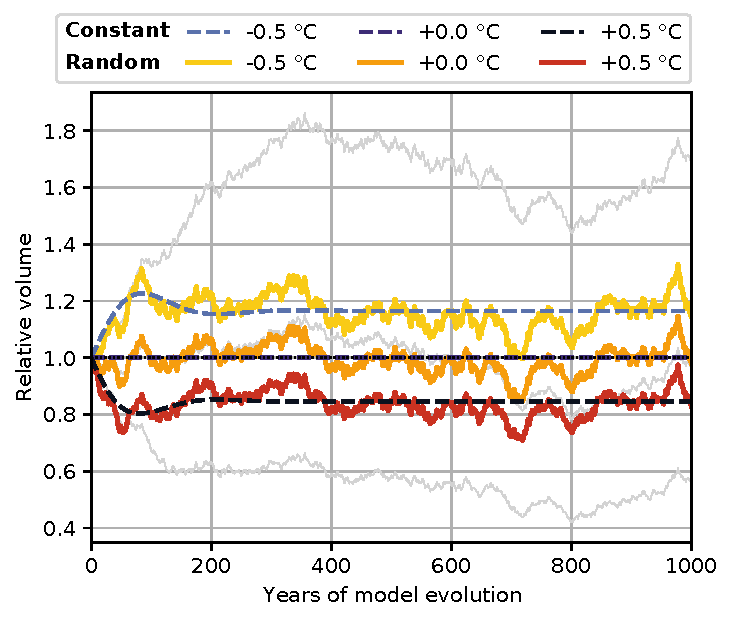
\includegraphics[width=\textwidth]{../plots/final_plots/time_series/single_glaciers/volume_norm_vas_Hintereisferner.pdf}
      \end{subfigure}
      \hfill
      % Flowline volume
      \begin{subfigure}[b]{0.476\textwidth}
        \caption{Flowline model, relative ice volume}
        \label{fig:hintereisferner:volume_fl}
        \centering
        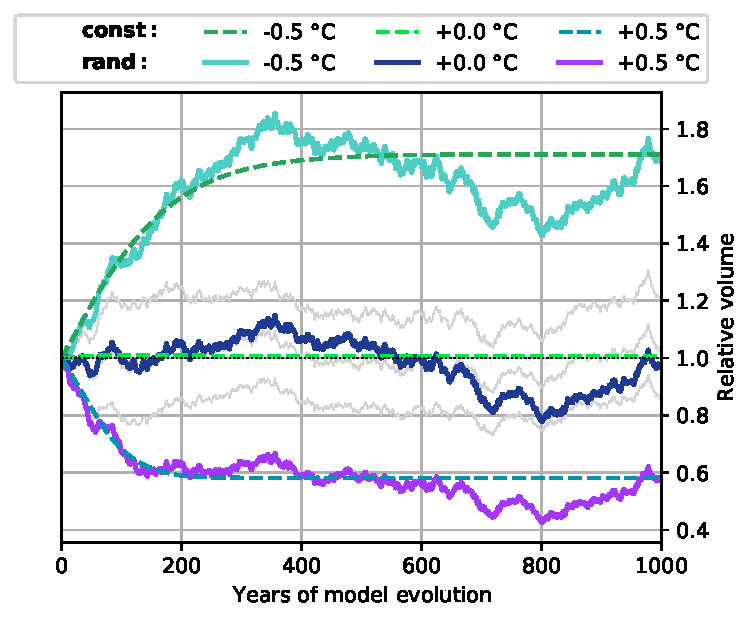
\includegraphics[width=\textwidth]{../plots/final_plots/time_series/single_glaciers/volume_norm_fl_Hintereisferner.pdf}
      \end{subfigure}

      % VAS area
      \begin{subfigure}[b]{0.476\textwidth}
        \caption{\Vas{} model, relative surface area}
        \label{fig:hintereisferner:area_vas}
        \centering
        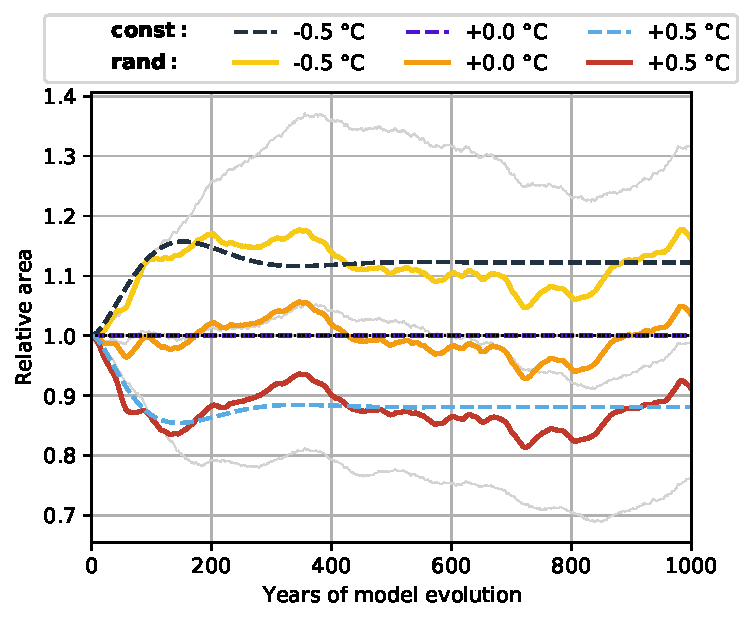
\includegraphics[width=\textwidth]{../plots/final_plots/time_series/single_glaciers/area_norm_vas_Hintereisferner.pdf}
      \end{subfigure}
      \hfill
      % Flowline area
      \begin{subfigure}[b]{0.476\textwidth}
        \caption{Flowline model, relative surface area}
        \label{fig:hintereisferner:area_fl}
        \centering
        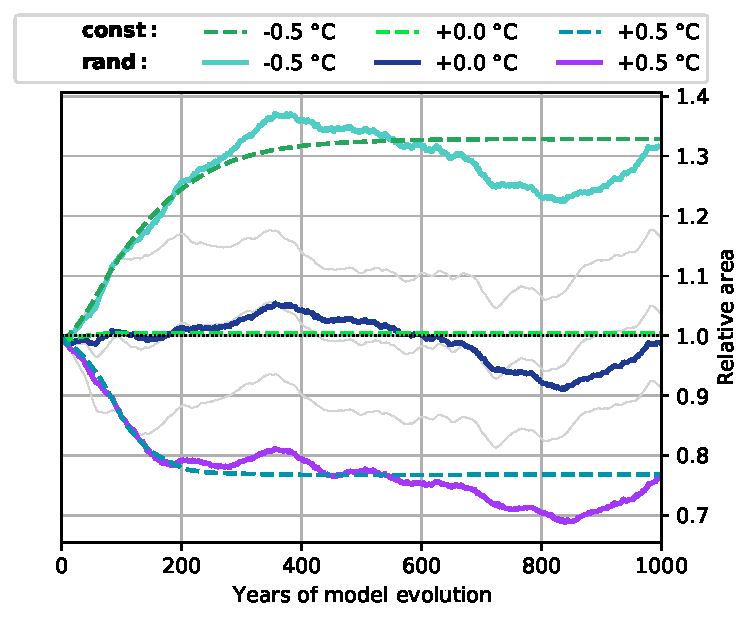
\includegraphics[width=\textwidth]{../plots/final_plots/time_series/single_glaciers/area_norm_fl_Hintereisferner.pdf}
      \end{subfigure}

      % VAS length
      \begin{subfigure}[b]{0.476\textwidth}
        \caption{\Vas{} model, relative glacier length}
        \label{fig:hintereisferner:length_vas}
        \centering
        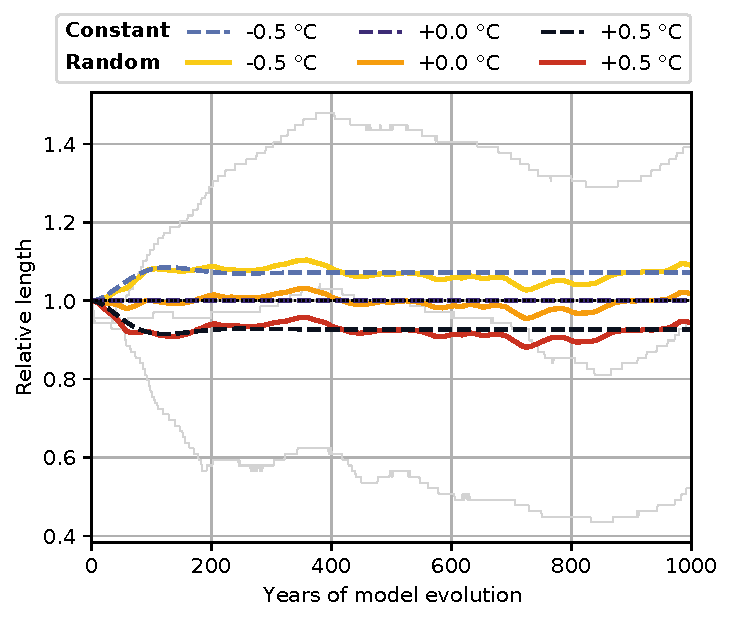
\includegraphics[width=\textwidth]{../plots/final_plots/time_series/single_glaciers/length_norm_vas_Hintereisferner.pdf}
      \end{subfigure}
      \hfill
      % Flowline length
      \begin{subfigure}[b]{0.476\textwidth}
        \caption{Flowline model, relative glacier length}
        \label{fig:hintereisferner:length_fl}
        \centering
        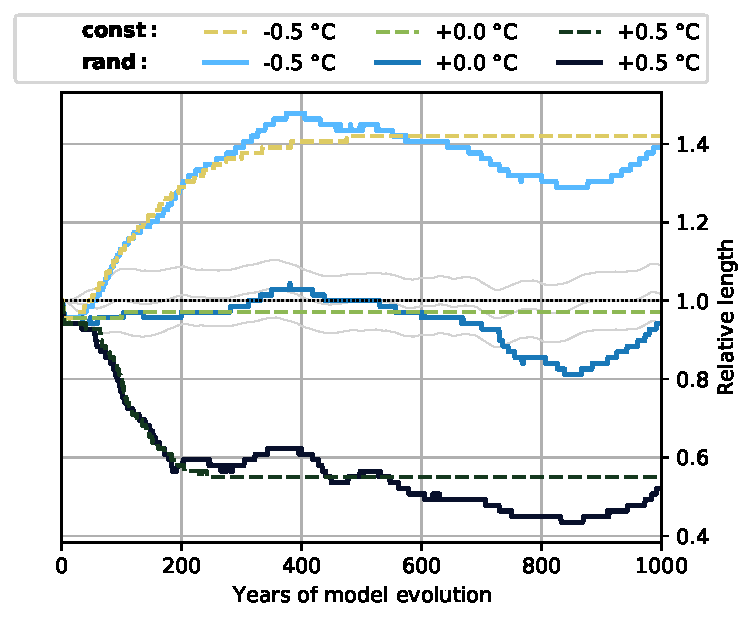
\includegraphics[width=\textwidth]{../plots/final_plots/time_series/single_glaciers/length_norm_fl_Hintereisferner.pdf}
      \end{subfigure}
      
      \caption{Temporal evolution of ice volume in (\subref{fig:hintereisferner:volume_vas}) and (\subref{fig:hintereisferner:volume_fl}), surface area in (\subref{fig:hintereisferner:area_vas}) and (\subref{fig:hintereisferner:area_fl}) and glacier length in (\subref{fig:hintereisferner:length_vas}) and (\subref{fig:hintereisferner:length_fl}) for Hintereisferner (RGI60-11.00897). The shown values area normalized with their respective initial values. The left panels show the result of the \vas{} model, the right panels show the results of the flowline model. Solid lines represent the random climate scenarios, while dashed lines represent the constant climate scenarios. All climate scenarios are based on an equilibrium climate. The applied temperature biases of \SI{-.5}{\celsius}, \SI{0}{\celsius} and \SI{+.5}{\celsius} are color coded, see legend for details. The dotted line indicates the initial volume. The light gray lines represent the volume evolutions of the other model, to facilitate comparisons.}
      \label{fig:hintereisferner}
    \end{figure}

    While the

  % section single_glacier_test_case_results (end)


  \section{Autocorrelation function and Power spectral density} % (fold)
  \label{sec:autocorrelation_and_power_spectral_density_results}
    
    % intro
    The autocorrelation function (ACF), partial autocorrelation function (PACF) and power spectral density (PSD) give insight into the periodicity and dominant frequencies of a given signal. The length signals of different  glaciers, modeled as response to different constant climate scenarios with random year-to-year variabilities, are investigated in this section (see Figure~\ref{fig:random_length}). The experiment is setup in analogy to the single glacier test case, since ACF, PACF and PSD are only meaningful for time series of a single glacier. To avoid a N-of-1 experiment, five more individual glaciers are investigated, namely the Pasterze, Mer de Glace, Glacier d'Argentière, Aletschgletscher and Rhonegletscher. All glaciers are subjected to different random (white noise) climate conditions for 20\ 000 years. The spinup period during which the glaciers adjust to the different climate is clipped, which leaves three different sizes of the same glacier. Hence, the temperature bias can be seen as a label for glacier size rather than climatic conditions. For details about the experimental setup see Section~\ref{sub:autocorrelation_and_power_spectral_density_setup}. The ACF for lag times up to 200 years is shown in Figure~\ref{fig:acf}, the PACF for lag times up to 20 years in Figure~\ref{fig:pacf} and the PSD in Figure~\ref{fig:psd}.

    Figure~\ref{fig:random_length} shows the length anomalies with respect to the equilibrium value for the arbitrarily chosen period between 8000 and 12\,000 years. This allows to formulate some first qualitative conclusions. The overlaid length changes seem to be in good agreement between the \vas{} and the flowline model. While correlations may be high, the difference in absolute length fluctuations is already apparent by looking at the y-scales (left for the flowline model and right for the \vas{} model). While the length changes estimated by the \vas{} model are all in the order of \SI{\pm200}{\meter} (except \SI{\pm500}{\meter} for the Pasterze, see Figure~\ref{fig:random_length:pasterze}), the flowline model predicts fluctuations between \SI{\pm500}{\meter} for the Rhonegletscher (Figure~\ref{fig:random_length:rhonegletscher}) and \SI{\pm2500}{\meter} for the Aletschgletscher (Figure~\ref{fig:random_length:großer_aletschgletscher}). Furthermore, different sizes of the same glacier show similar but noticeable different length fluctuation under the flowline model, while there seems to be little to no differences under the \vas{} model. However, these first findings are only based on the visual inspection of a temporally limited subsample and are further investigated and quantified in the following sections.

    \subsection{Power spectral density} % (fold)
    \label{sub:power_spectral_density_results}

      % intro and general
      % low pass filter
      Glaciers act as low-pass filters for the natural climate variability. A low pass filter passes lower frequencies while attenuating higher frequencies, which results in a characteristic PSD curve. Figure~\ref{fig:psd} shows the PSD of glacier lengths for the six glaciers mentioned above. The power density stays in a constant range for frequencies up to \SI{3e-3}{\per\year} (corresponding to signals with a period of over 300 years) before decreasing with increasing frequency. This makes intuitive sense, since changes in glacier length are mainly driven by long term climatic trends and less by inter-annual variabilities in the climatic forcing. A single year with low temperatures and strong (cold season) precipitation has less impact on the glacier size than a decade of slightly above-average temperatures.
      % higher power density of flowline model
      While the overall shape of the PSDs are similar for the \vas{} model and the flowline model, there are some key differences. As seen before, the length changes estimated by the \vas{} model are smaller compared to the flowline model. Hence, the overall power of the flowline model is higher across all frequencies. In agreement with the symmetric behavior discussed before, the PSDs of the \vas{} model are practically identical for different sizes of the same glacier. The PSDs based on the flowline length are less coherent between different sizes of the same glacier, whereby there is no discernible relation between shape of PSD and glacier size.
      % power density for high frequencies
      Additionally, the flowline model shows a rather constant power density for lower frequencies. This is due to the discrete changes in glacier length of the flowline model, whose resolution depends on the grid size (\SI{100}{\meter} in this case). The \vas{} model length is a continuous variable, resulting in a constantly decreasing power density.
      % slope?
      While the absolute values are different, the slope of the PSDs are almost identical between \vas{} and flowline model for medium frequencies up to about \SI{3e-2}{\per\year} (corresponding to signals with a period of over 30 years). This indicates that the breakdown of energy from larger to smaller scales happens at similar rates for both models (cp. the energy cascade for turbulent flows, e.g., \cite{Wyngaard2010}).

      % Random length plots
      \begin{figure}[htp]
        \centering
        \begin{subfigure}[b]{0.48\textwidth}
          \caption{RGI60-11.00897 - Hintereisferner}
          \label{fig:random_length:hintereisferner}
          \centering
          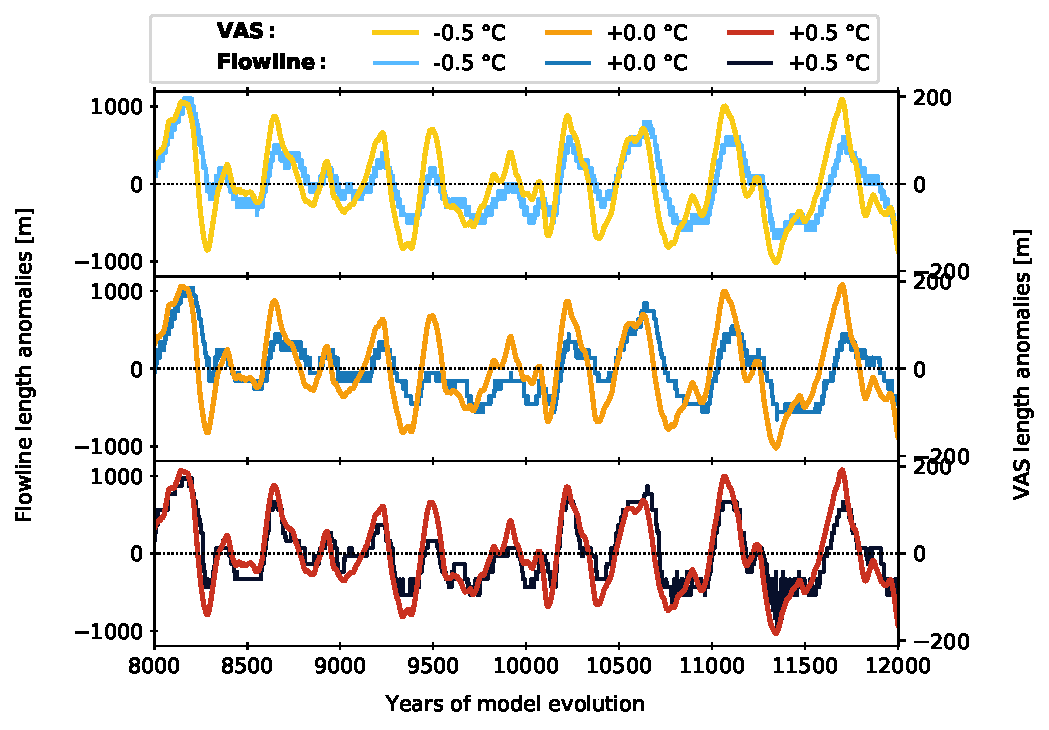
\includegraphics[width=\textwidth]{../plots/final_plots/random_length/Hintereisferner.pdf}
        \end{subfigure}
        \hfill
        \begin{subfigure}[b]{0.48\textwidth}
          \caption{RGI60-11.00106 - Pasterze}
          \label{fig:random_length:pasterze}
          \centering
          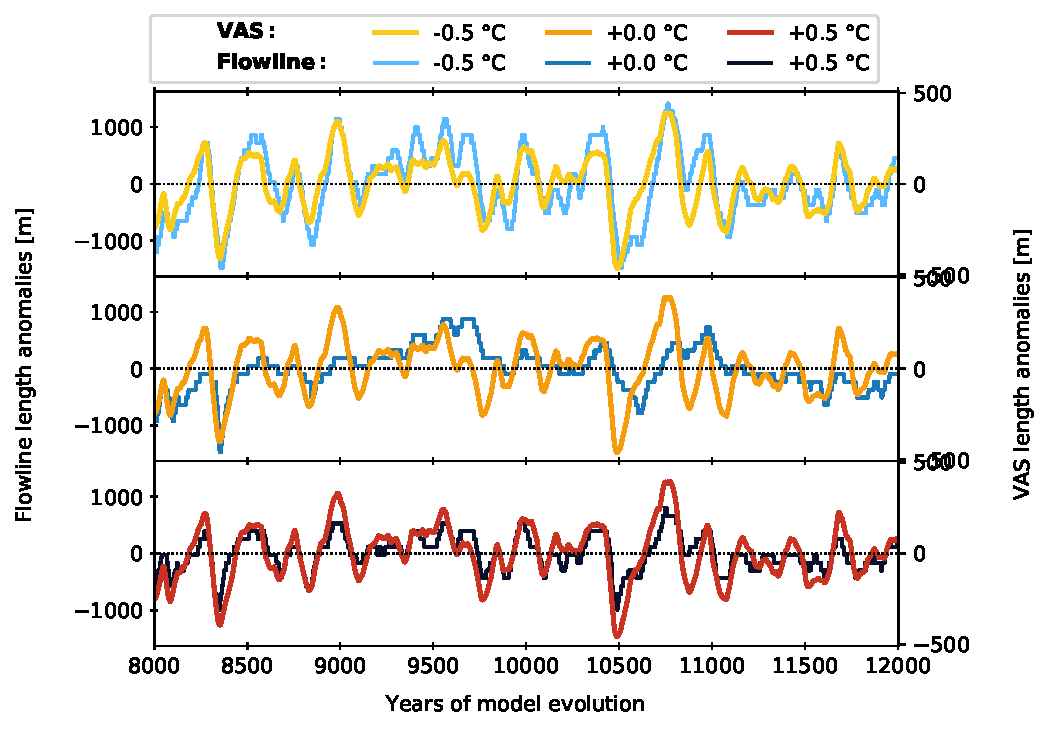
\includegraphics[width=\textwidth]{../plots/final_plots/random_length/Pasterze.pdf}
        \end{subfigure}
        \begin{subfigure}[b]{0.48\textwidth}
          \caption{RGI60-11.03643 - Mer de Glace}
          \label{fig:random_length:mer_de_glace}
          \centering
          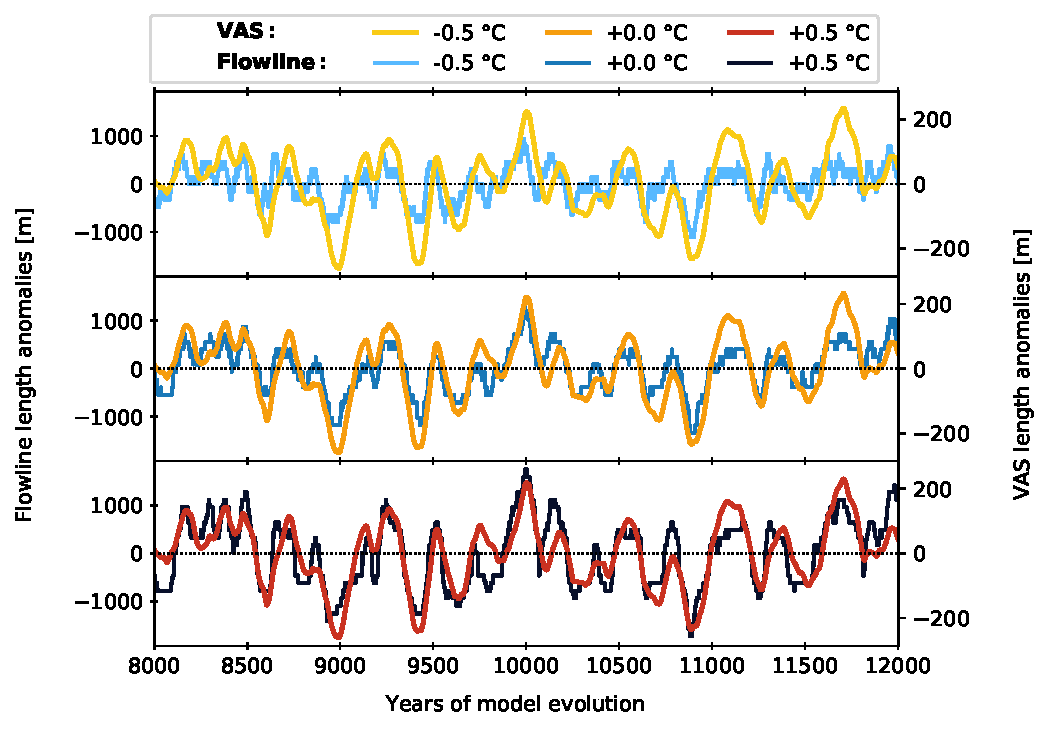
\includegraphics[width=\textwidth]{../plots/final_plots/random_length/Mer_de_Glace.pdf}
        \end{subfigure}
        \hfill
        \begin{subfigure}[b]{0.48\textwidth}
          \caption{RGI60-11.03638 - d'Argentière}
          \label{fig:random_length:glacier_d_argentiere}
          \centering
          \includegraphics[width=\textwidth]{../plots/final_plots/random_length/Glacier_d'Argentière.pdf}
        \end{subfigure}
        \begin{subfigure}[b]{0.48\textwidth}
          \caption{RGI60-11.01450 - Großer Aletschgletscher}
          \label{fig:random_length:großer_aletschgletscher}
          \centering
          \includegraphics[width=\textwidth]{../plots/final_plots/random_length/Großer_Aletschgletscher.pdf}
        \end{subfigure}
        \hfill
        \begin{subfigure}[b]{0.48\textwidth}
          \caption{RGI60-11.01238 - Rhonegletscher}
          \label{fig:random_length:rhonegletscher}
          \centering
          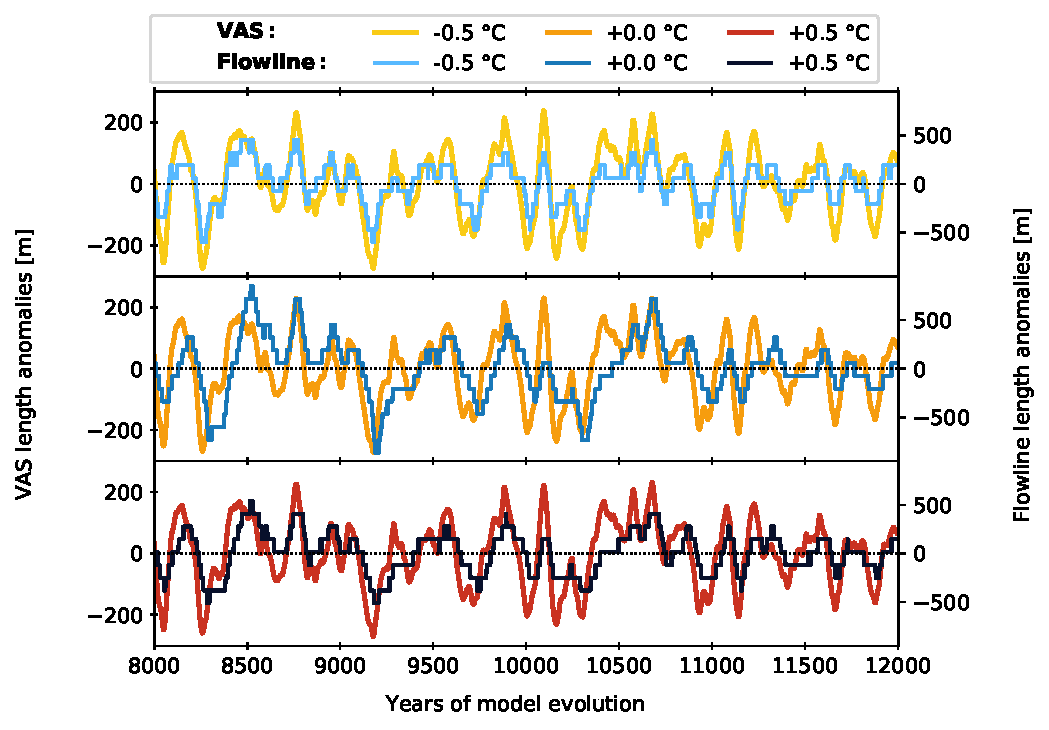
\includegraphics[width=\textwidth]{../plots/final_plots/random_length/Rhonegletscher.pdf}
        \end{subfigure}

        \caption{Length anomalies from to the respective average (equilibrium) value. The climate scenarios are based on a randomized equilibrium climate, with different temperature biases. Cyan, blue and purple lines represent the flowline model, while yellow, orange and red lines represent the \vas{} model, with a temperature bias of \SI{-.5}{\celsius}, \SI{0}{\celsius} and \SI{+.5}{\celsius}, respectively. Note the differences in y-axis scales.}
        \label{fig:random_length} 
      \end{figure}
      
      % PSD plots
      \begin{figure}[htp]
        \centering
        \begin{subfigure}[b]{0.48\textwidth}
          \caption{RGI60-11.00897 - Hintereisferner}
          \label{fig:psd:hintereisferner}
          \centering
          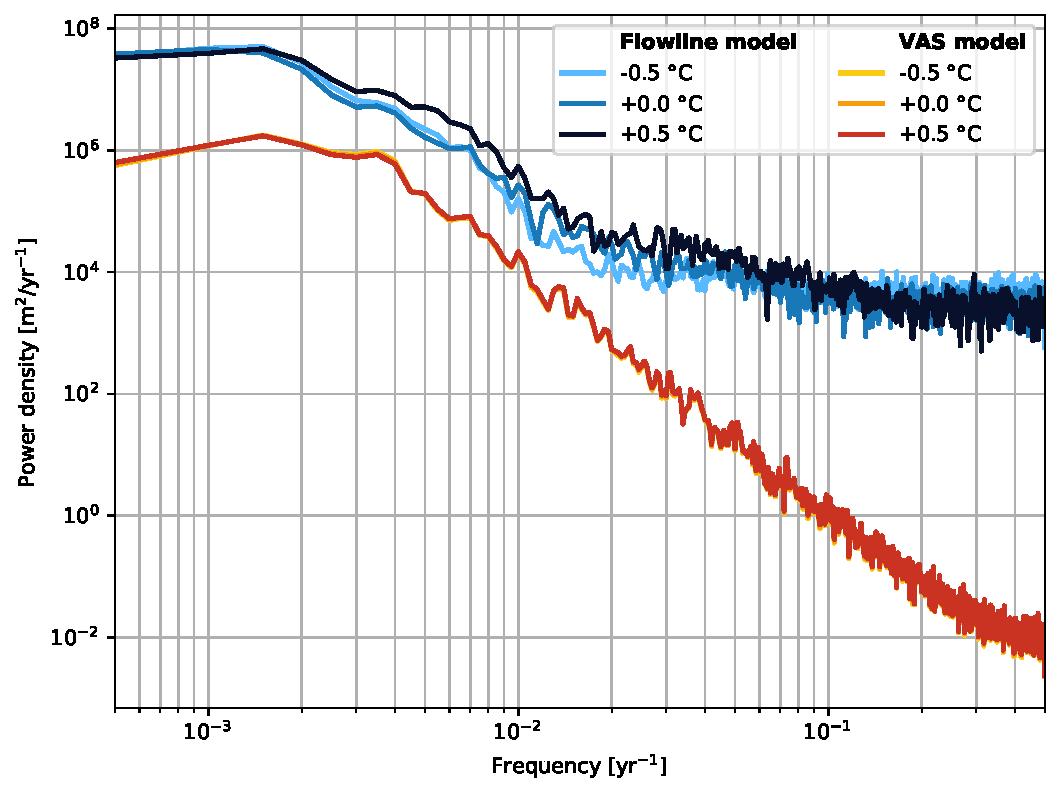
\includegraphics[width=\textwidth]{../plots/final_plots/psd/Hintereisferner.pdf}
        \end{subfigure}
        \hfill
        \begin{subfigure}[b]{0.48\textwidth}
          \caption{RGI60-11.00106 - Pasterze}
          \label{fig:psd:pasterze}
          \centering
          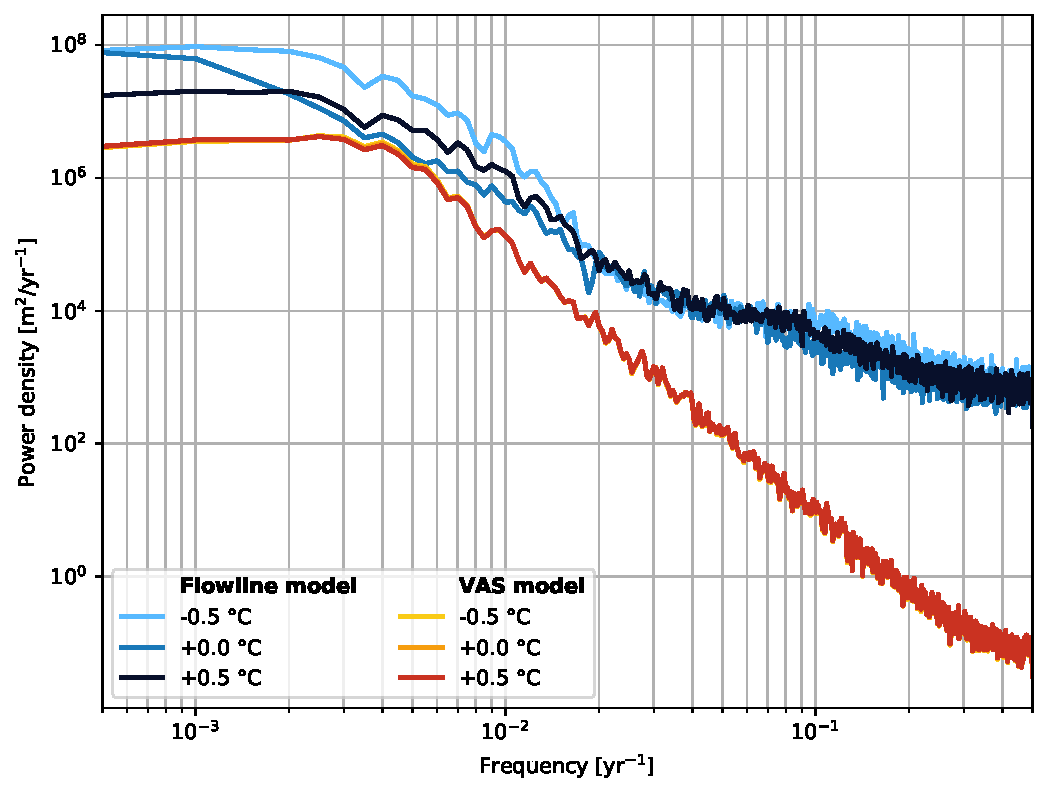
\includegraphics[width=\textwidth]{../plots/final_plots/psd/Pasterze.pdf}
        \end{subfigure}
        \begin{subfigure}[b]{0.48\textwidth}
          \caption{RGI60-11.03643 - Mer de Glace}
          \label{fig:psd:mer_de_glace}
          \centering
          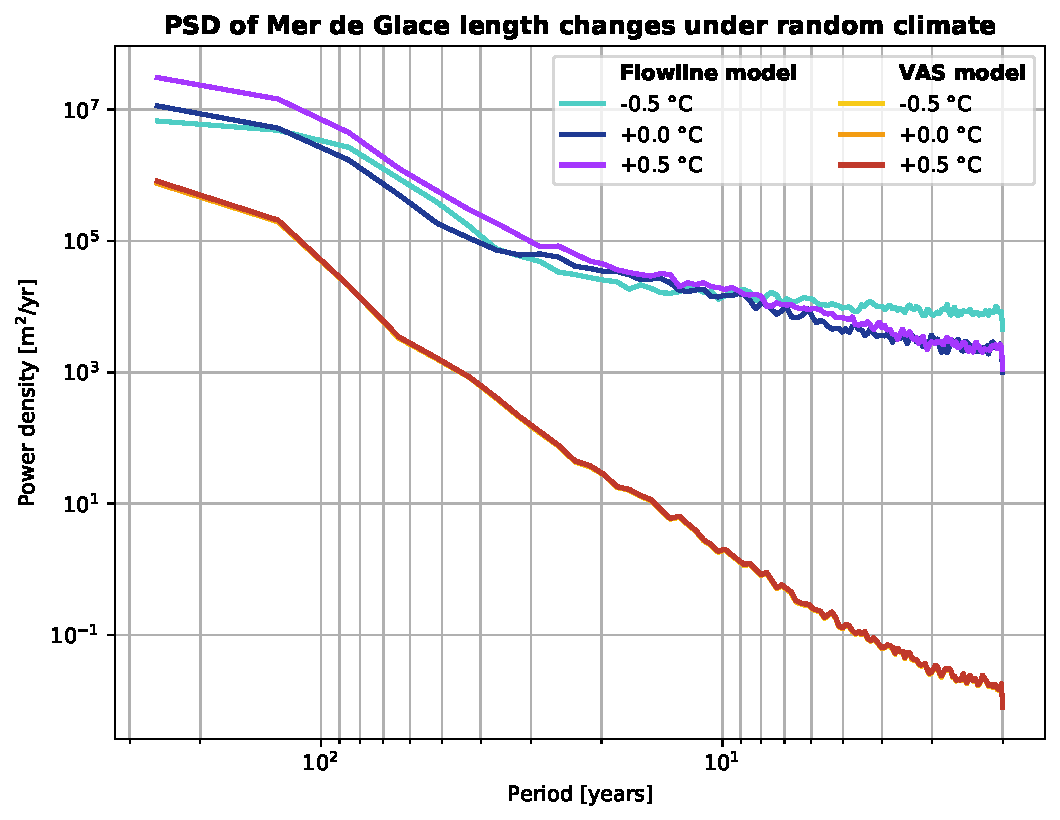
\includegraphics[width=\textwidth]{../plots/final_plots/psd/Mer_de_Glace.pdf}
        \end{subfigure}
        \hfill
        \begin{subfigure}[b]{0.48\textwidth}
          \caption{RGI60-11.03638 - d'Argentière}
          \label{fig:psd:glacier_d_argentiere}
          \centering
          \includegraphics[width=\textwidth]{../plots/final_plots/psd/Glacier_d'Argentière.pdf}
        \end{subfigure}
        \begin{subfigure}[b]{0.48\textwidth}
          \caption{RGI60-11.01450 - Großer Aletschgletscher}
          \label{fig:psd:großer_aletschgletscher}
          \centering
          \includegraphics[width=\textwidth]{../plots/final_plots/psd/Großer_Aletschgletscher.pdf}
        \end{subfigure}
        \hfill
        \begin{subfigure}[b]{0.48\textwidth}
          \caption{RGI60-11.01238 - Rhonegletscher}
          \label{fig:psd:rhonegletscher}
          \centering
          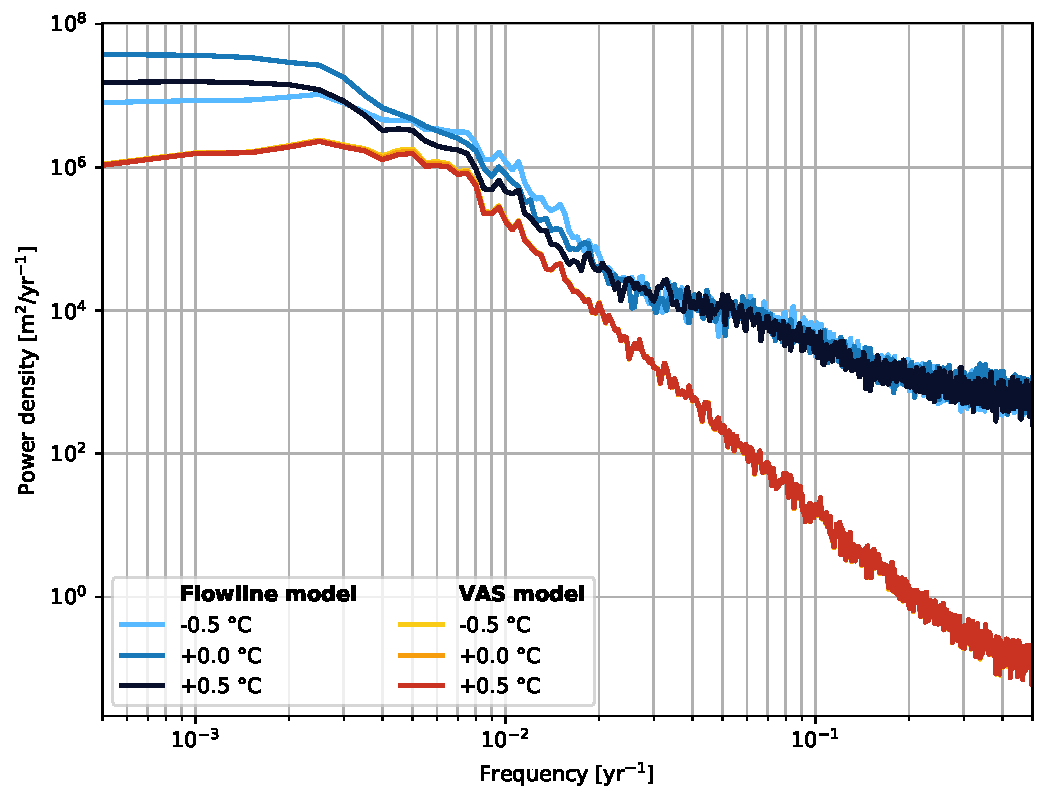
\includegraphics[width=\textwidth]{../plots/final_plots/psd/Rhonegletscher.pdf}
        \end{subfigure}

        \caption{Power spectral density of modeled glacier length for different alpine glaciers. Different lines represent different combinations of evolution models and climate scenarios. The climate scenarios are based on a randomized equilibrium climate, with different temperature biases. Cyan, blue and purple lines represent the flowline model, while yellow, orange and red lines represent the \vas{} model, with a temperature bias of \SI{-.5}{\celsius}, \SI{0}{\celsius} and \SI{+.5}{\celsius}, respectively. Note the differences in y-axis scales.}
        \label{fig:psd}
      \end{figure}
    
    % subsection power_spectral_density_results (end)

    \subsection{Autocorrelation function} % (fold)
    \label{sub:autocorrelation_function_results}

      A general observation about the ACF can be made for both models, all glaciers and climate scenarios: the correlation is high for the first few lag times, before it decreases exponentially. This points at an autoregressive (AR) term and a moving-average (MA) term in the data. An autoregressive-moving-average model (ARMA) predicts future values of a random variable based on a linear combination of the past values and past error terms of said variable. This makes intuitive sense for glaciers, since the past and current glacier size and the difference to the equilibrium value have a direct influence on next years glacier size. A more detailed discussion of a potential ARMA model is provided at the end of this section.

      Same as for the PSDs, the ACFs for the \vas{} length signals are almost identical between different sizes of the same glacier, indicating that the glacier size has little to no effect on the transient behavior of the model. The \vas{} model represents the glacier as a simple cuboid without any additional information about the glacier shape. The absolute dimensions of that cuboid seem to have less of an effect on the ACF than other parameters, which differe from glacier to glacier. Some glaciers, like the Glacier d'Argentière and the Aletschgletscher show statistically significant negative correlations for higher lag terms between 80 and 250 years, while the others show very little to no significant negative correlation for higher lag times. However, no apparent relation between the strength of negative correlations for later lag times and any other glacier parameter, like the average slope or the model-internal lag times, was found.
      The average slope is the only additional geometric information of the \vas{} model, even if it is implemented only indirectly. The slope is independent of the glacier's sizes. However, it affects the temporal evolution, since changes in terminus elevation---and thereby changes in specific mass balance---are linearly related to changes in glacier length. This can be seen in the ACF plots, which vary from glacier to glacier but not between different sizes of the same glacier.  However, their is no obvious pattern when comparing the ACF to the average slope\footnote{Possible future work could include a in-depth investigation on how glacier characteristics influence its ACF. Thereby, the ACF could add information, or even superseed, to the concept of e-folding response times as glacier characteristics.}.
    
      The flowline model is able to represent different glacier geometries and grasp individual responses under different equilibrium climates, which can be seen in the vastly different ACFs. They differ from glacier to glacier, but also for different sizes of the same glacier. However, there are again no discernible patterns, which confirms the notion that the flowline model is capable of simulating each glacier's individual response. The autocorrelation of the flowline model is generally stronger than for the \vas{} runs for most glaciers and most temperature biases, even though not for all. The following list points to some particular observations:
      \begin{itemize}
        \item for Hintereisferner (Figure~\ref{fig:acf:hintereisferner}) the ACFs of the flowline model show higher correlations than for the \vas{} model, while for Mer de Glace (Figure~\ref{fig:acf:mer_de_glace}) and Großer Aletschgletscher (Figure~\ref{fig:acf:großer_aletschgletscher}) the flowline model ACFs show equal ore lower correlations for lag time up to around fifty years;
        \item the flowline model of the Pasterze (Figure~\ref{fig:acf:pasterze}) shows a strong autocorrelation under the equilibrium climate, i.e., for its medium size, ($r>0.6$ for lags times up to one-hundred years and statistically significant up until a lag time of 243 years), while under a warmer and colder equilibrium climate (\SI{\pm0.5}{\celsius}) the autocorrelation of all lag times is comparable to the \vas{} model;
        \item similarly, the flowline model of the Glacier d'Argentière (Figure~\ref{fig:acf:glacier_d_argentiere}) shows a strong autocorrelation under the warmer equilibrium climate (\SI{+0.5}{\celsius}), while the autocorrelation under the other two climate scenarios is even lower than the ACF of the \vas{} model.
      \end{itemize}
      The only observation made for all glaciers, it that the \vas{} model shows a stronger or equal autocorrelation for shorter lag time (i.e., less than about twenty years) than the flowline model. This is true even for glaciers, where the autocorrelation of the flowline mode is generally stronger than for the \vas{} model (e.g., Hintereisferner).

      Strong correlations for short lag times influences the correlation of all following lag terms. For example, an exponentially decaying signal, which halves its value with each time step $\Phi(t) = 0.5 \Phi(t-1)$, will have an autocorrelation of 0.5 for lag 1, 0.25 for lag 2, 0.125 for lag 3, and so on. Depending on the sample size these values will be statistically significant, even though only one lag term is included in the definition of the signal (i.e., an AR(1) process). The partial autocorrelation function (PACF) measures only these direct influences, eliminating the effects of all shorter lag times. All the PACFs of the \vas{} model lengths show a strong positive correlation for lag times of 1 year, followed by a strong negative correlation which then slowly increases towards zero. Correlations for lag times ten and greater are not, or only marginally, significant. Again, there are no discernible differences between different sizes of the same glacier and very little differences from one glacier to another. The PACFs for the flowline model lengths show the same high correlation for the lag time of one year, before decreasing towards zero. The decrease towards statistical insignificant correlations happens quite fast for most glaciers. Only Mer de Glace (Figure~\ref{fig:pacf:mer_de_glace}) and Glacier d'Argentière (Figure~\ref{fig:pacf:glacier_d_argentiere}), both for the warmer climate, and Rhonegletscher (Figure~\ref{fig:pacf:rhonegletscher}), for the equilibrium climate, show significant correlations for lag times greater than three years. For higher lag times between ten and twenty years there are some negative correlations, even though they are only marginally significant.

      The number of statistically significant terms of the PACF informs on the order $p$ for the AR($p$) model. The order specifies the of number lag terms that are considered. Analogously, the order $q$ for the MA($q$) model can be estimated from the number of significant terms of the ACF. By this definition, the \vas{} model could be ... by an ARMA(9, 70) model, and the flowline model by an ARMA(3, 140). Hereby, the orders are taken as average over all glaciers and climate scenarios (see Appendix~\ref{appendix_B} for details). While an AR model with nine lag terms would be big but still feasible, a MA model with over one-hundred lag terms is neither practicable nor does it make sense. Especially, since \citet{Roe2014} use an ARMA(3,3) model to produce comparable results to a flowline model. It is not the intent of this work to investigate the relation between a glacier's geometry and its ACF, neither to fit an ARMA model to the data. Hence, this qualitative first look has to suffice. However, it is most notable that the flowline model behaves differently not only for different glaciers, but also for different sizes of the same glacier. The \textit{one size fits all} approach of the \vas{} model produces more homogeneous results, the ACFs and PACFs are mostly independent of a glacier's size.

      \begin{figure}[htp]
        \centering
        
        \begin{subfigure}[b]{0.48\textwidth}
          \caption{RGI60-11.00897 - Hintereisferner}
          \label{fig:acf:hintereisferner}
          \centering
          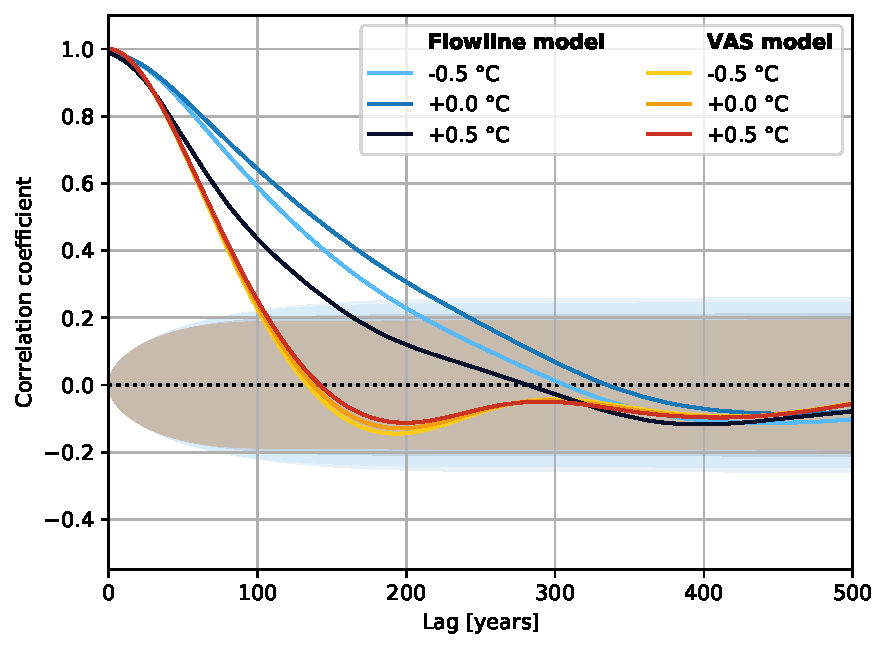
\includegraphics[width=\textwidth]{../plots/final_plots/acf/Hintereisferner.pdf}
        \end{subfigure}
        \hfill
        \begin{subfigure}[b]{0.48\textwidth}
          \caption{RGI60-11.00106 - Pasterze}
          \label{fig:acf:pasterze}
          \centering
          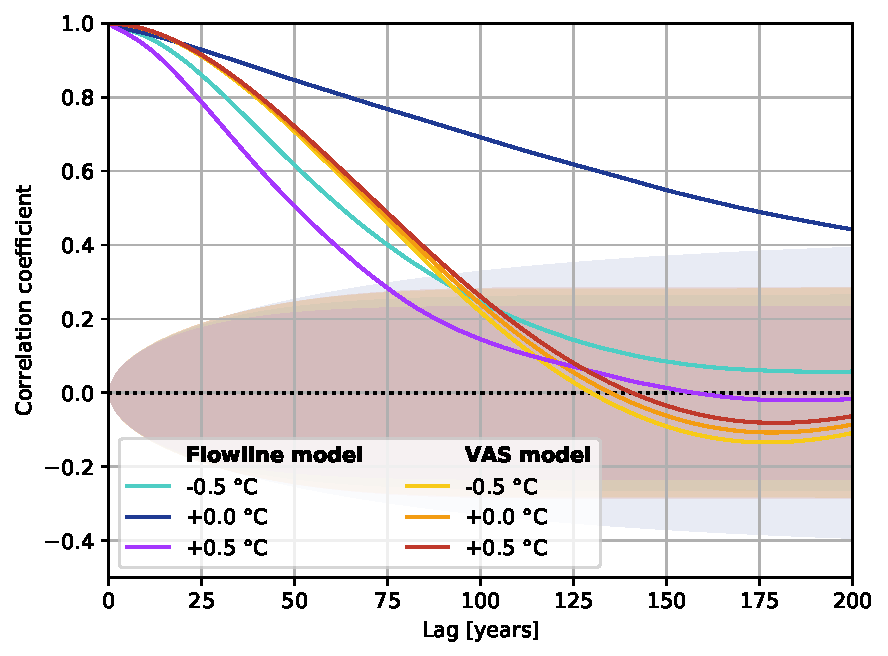
\includegraphics[width=\textwidth]{../plots/final_plots/acf/Pasterze.pdf}
        \end{subfigure}

        \begin{subfigure}[b]{0.48\textwidth}
          \caption{RGI60-11.03643 - Mer de Glace}
          \label{fig:acf:mer_de_glace}
          \centering
          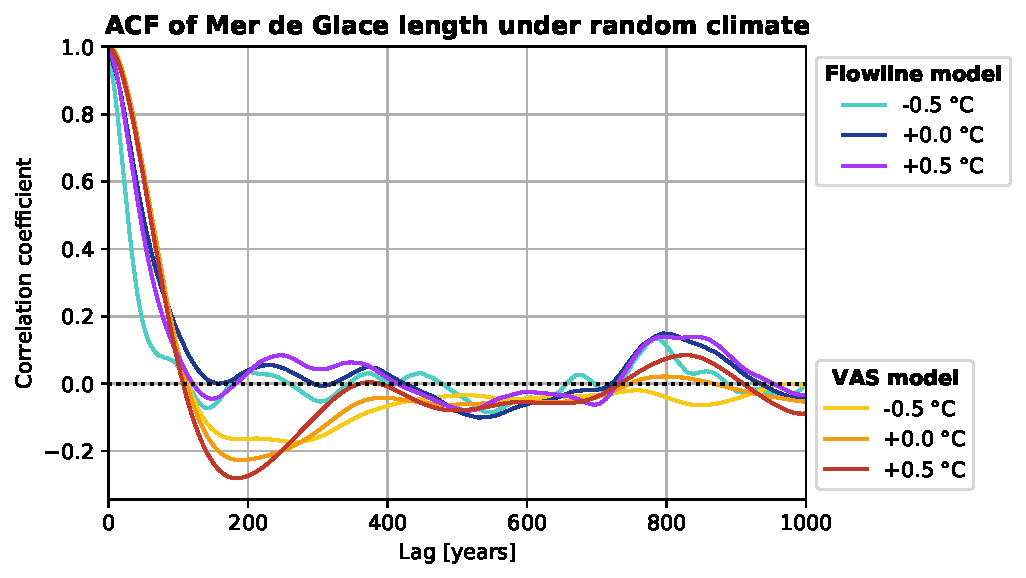
\includegraphics[width=\textwidth]{../plots/final_plots/acf/Mer_de_Glace.pdf}
        \end{subfigure}
        \hfill
        \begin{subfigure}[b]{0.48\textwidth}
          \caption{RGI60-11.03638 - d'Argentière}
          \label{fig:acf:glacier_d_argentiere}
          \centering
          \includegraphics[width=\textwidth]{../plots/final_plots/acf/Glacier_d'Argentière.pdf}
        \end{subfigure}

        \begin{subfigure}[b]{0.48\textwidth}
          \caption{RGI60-11.01450 - Großer Aletschgletscher}
          \label{fig:acf:großer_aletschgletscher}
          \centering
          \includegraphics[width=\textwidth]{../plots/final_plots/acf/Großer_Aletschgletscher.pdf}
        \end{subfigure}
        \hfill
        \begin{subfigure}[b]{0.48\textwidth}
          \caption{RGI60-11.01238 - Rhonegletscher}
          \label{fig:acf:rhonegletscher}
          \centering
          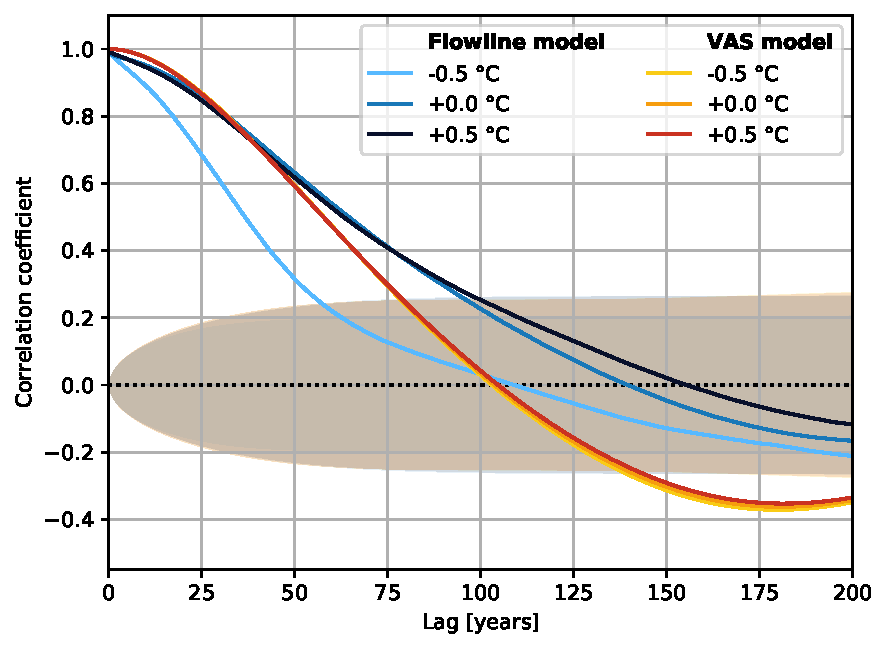
\includegraphics[width=\textwidth]{../plots/final_plots/acf/Rhonegletscher.pdf}
        \end{subfigure}

        \caption{Autocorrelation function of modeled length for lag times between zero and 200 years. Different lines represent different combinations of evolution model and climate scenario.
        The random climate scenario is based on an equilibrium climate, with different temperature biases.
        Cyan, blue and purple lines represent the flowline model, while yellow, orange and red lines represent the \vas{} model, with a temperature bias of \SI{-.5}{\celsius}, \SI{0}{\celsius} and \SI{+.5}{\celsius}, respectively.
        The \SI{99}{\percent} confidence intervals are shaded in the corresponding colors.}
        \label{fig:acf}
      \end{figure}

      \begin{figure}[htp]
        \centering
        
        \begin{subfigure}[b]{0.48\textwidth}
          \caption{RGI60-11.00897 - Hintereisferner}
          \label{fig:pacf:hintereisferner}
          \centering
          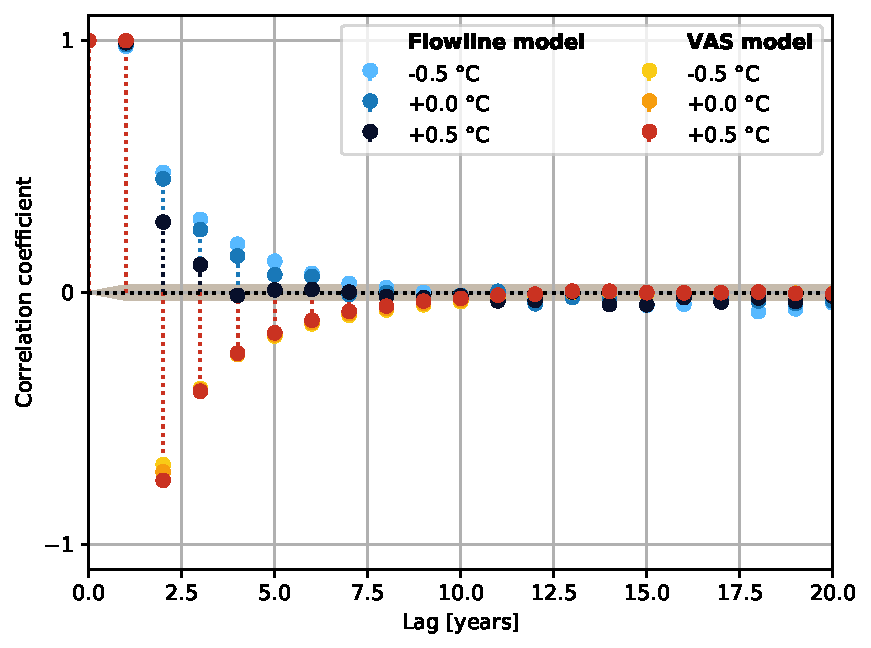
\includegraphics[width=\textwidth]{../plots/final_plots/pacf/Hintereisferner.pdf}
        \end{subfigure}
        \hfill
        \begin{subfigure}[b]{0.48\textwidth}
          \caption{RGI60-11.00106 - Pasterze}
          \label{fig:pacf:pasterze}
          \centering
          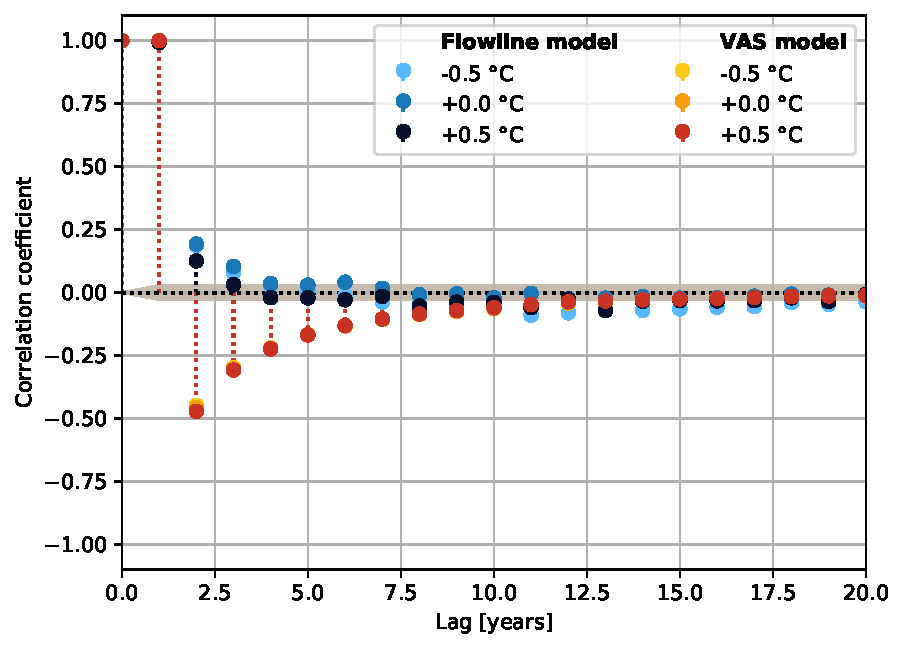
\includegraphics[width=\textwidth]{../plots/final_plots/pacf/Pasterze.pdf}
        \end{subfigure}

        \begin{subfigure}[b]{0.48\textwidth}
          \caption{RGI60-11.03643 - Mer de Glace}
          \label{fig:pacf:mer_de_glace}
          \centering
          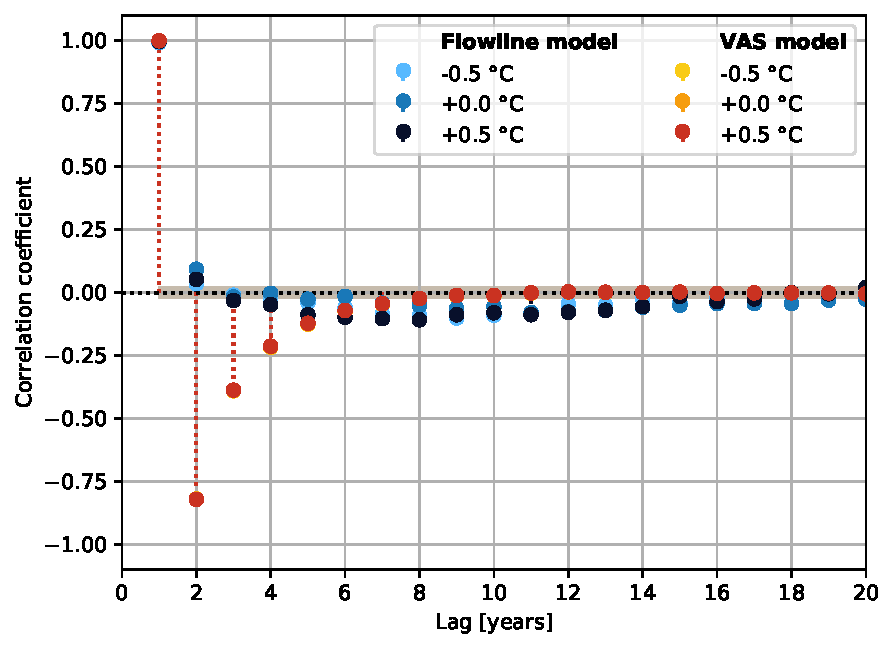
\includegraphics[width=\textwidth]{../plots/final_plots/pacf/Mer_de_Glace.pdf}
        \end{subfigure}
        \hfill
        \begin{subfigure}[b]{0.48\textwidth}
          \caption{RGI60-11.03638 - d'Argentière}
          \label{fig:pacf:glacier_d_argentiere}
          \centering
          \includegraphics[width=\textwidth]{../plots/final_plots/pacf/Glacier_d'Argentière.pdf}
        \end{subfigure}

        \begin{subfigure}[b]{0.48\textwidth}
          \caption{RGI60-11.01450 - Großer Aletschgletscher}
          \label{fig:pacf:großer_aletschgletscher}
          \centering
          \includegraphics[width=\textwidth]{../plots/final_plots/pacf/Großer_Aletschgletscher.pdf}
        \end{subfigure}
        \hfill
        \begin{subfigure}[b]{0.48\textwidth}
          \caption{RGI60-11.01238 - Rhonegletscher}
          \label{fig:pacf:rhonegletscher}
          \centering
          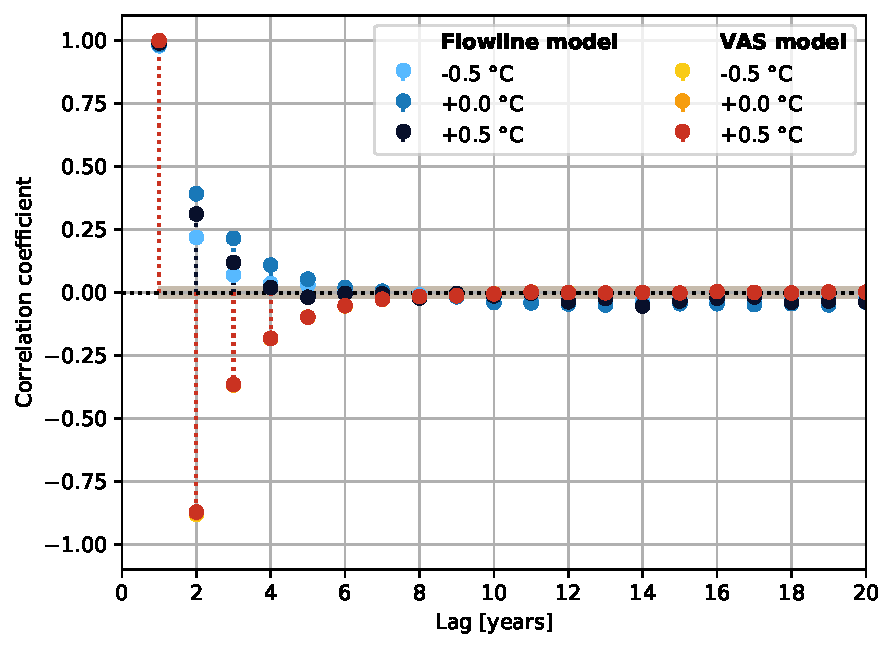
\includegraphics[width=\textwidth]{../plots/final_plots/pacf/Rhonegletscher.pdf}
        \end{subfigure}

        \caption{Partial autocorrelation function of modeled length for lag times between zero and 200 years. Different lines represent different combinations of evolution model and climate scenario.
        The random climate scenario is based on an equilibrium climate, with different temperature biases.
        Cyan, blue and purple lines represent the flowline model, while yellow, orange and red lines represent the \vas{} model, with a temperature bias of \SI{-.5}{\celsius}, \SI{0}{\celsius} and \SI{+.5}{\celsius}, respectively.
        The \SI{99}{\percent} confidence intervals are shaded in the corresponding colors.}
        \label{fig:pacf}
      \end{figure}

    % subsection autocorrelation_function_results (end)

  % section autocorrelation_fand_power_spectral_density_results (end)

  \section{Regional runs with all Alpine glaciers} % (fold)
  \label{sec:regional_runs_with_all_alpine_glaciers_results}

    \Vas{} should not be applied to individual glaciers, but only to populations of glaciers \citep{Bahr2015}, where the scaling approach shows its strength: the law of large number assures a reasonable estimation of the collective glacier ice volume, since random errors will be canceled out by each other. This section compares the behavior of the \vas{} model to the flowline model, on the example of all Alpine glaciers under different climate scenarios (analogous to the single glacier test case, see Section~\ref{sec:single_glacier_test_case_results}).
    Again, both mass balance models simulate different climate scenarios with the same three temperature biases as above, based on the equilibrium period centered around \lstinline`y0` = \tstar{}. The only difference to the single glacier test case is that the \vas{} model and the flowline model each use their respective \tstar{} reference tables. For more details about the experimental setup see Section~\ref{sub:regional_runs_with_all_alpine_glaciers_setup}. The time series plots of normalized and absolute total Alpine ice volume are shown in Figure~\ref{fig:histalp_commitment}.

    Both evolution models run for 1000 years with the \lstinline`ConstantMassBalance` model and the \lstinline`RandomMassBalance` model. The random climate with its year-to-year fluctuations is obviously more physical than the completely constant climate. However, the resulting changes in glacier ice volume under both climate scenarios are almost identical. This makes intuitive sense, considering that glaciers act as natural low-pass filters for climatic variabilities (as established above, see Section~\ref{sub:power_spectral_density_results}). Short term climatic variabilities have little to no effect on the ice volume of a single glacier, much less on the aggregate ice volume of an entire region. Over the last 200 years of the simulations, the relative differences in aggregate ice volume between the constant and random climate scenario never exceed \SI{0.6}{\percent} for the \vas{} model and \SI{1.7}{\percent} for the flowline model. Only the \SI{0}{\celsius}-run of flowline model shows higher relative differences, with an average of \SI{2.0}{\percent} over the last 200 years, up to a maximum of \SI{2.7}{\percent}. While the total ice volume stays close to it's initial value, it shows a slight increase over time. After an initially strong increase of \SI{1.6}{\percent} over the first fifty years and another fifty years of constant values, the volume grows almost linearly with about \SI{0.53}{\cubic\kilo\meter} per 100 years under the constant climate scenario. This results in a total volume change of \SI{5.6}{\cubic\kilo\meter} (\SI{+3.4}{\percent} of the initial value) after 1000 years of simulation. Under the random climate scenario, the total ice volume grows slower, most likely since the oscillations will reduce certain feedback loops. Long story short, the following discussion is simplified by only considering the constant climate scenarios. 

    The \vas{} model estimates a total Alpine ice volume of \SI{156}{\cubic\kilo\meter} (\SI{+20}{\percent}), \SI{130}{\cubic\kilo\meter} (\SI{\pm{}0}{\percent}) and \SI{109}{\cubic\kilo\meter} (\SI{-17}{\percent}), while the flowline model estimates a total Alpine ice volume of \SI{259}{\cubic\kilo\meter} (\SI{+59}{\percent}), \SI{169}{\cubic\kilo\meter} (\SI{+3}{\percent}) and \SI{92}{\cubic\kilo\meter} (\SI{-44}{\percent}), after 1000 years of simulation under a temperature bias of \SI{-0.5}{\celsius}, \SI{0}{\celsius} and \SI{+0.5}{\celsius}, respectively.

    All the general characteristics of the \vas{} model found for the Hintereisferner test case turn up again for the regional. The \vas{} scaling model underestimates the changes in ice volume compared to the flowline model by a factor of \num{\approx 3.5}. The oscillatory behavior of the \vas{} model is still visible The \vas{} model's response time scales to the step changes in climate are shorter that for the flowline model. The volume e-folding time scales of both models are comparable to the single glacier test case: $\tau_V = \SI{23}{\year}$ and $\tau_V = \SI{20}{\year}$ for the \vas{} model and $\tau_V = \SI{125}{\year}$ and $\tau_V = \SI{79}{\year}$ for the flowline model, for the negative and positive temperature perturbation, respectively. These values are highly influenced by the larger glaciers and serve only as a guidance level. The symmetric behavior of the \vas{} model is still reflected in the response times, but less so in the new equilibrium values.

    All in all, the \vas{} model does a bad job compared to the flowline model, even though no statement about the model accuracy can be made without any comparison to observational data. The next section explores the possibilities of tuning the \vas{} model via different parameters for the used scaling relations. This also provides a range of plausible results and serves as uncertainty estimation.

    \begin{figure}[htp]
      \centering
      \begin{subfigure}[b]{0.48\textwidth}
        \caption{\Vas{} model, relative glacier volume}
        \label{fig:histalp_commitment:volume_norm_const}
        \centering
        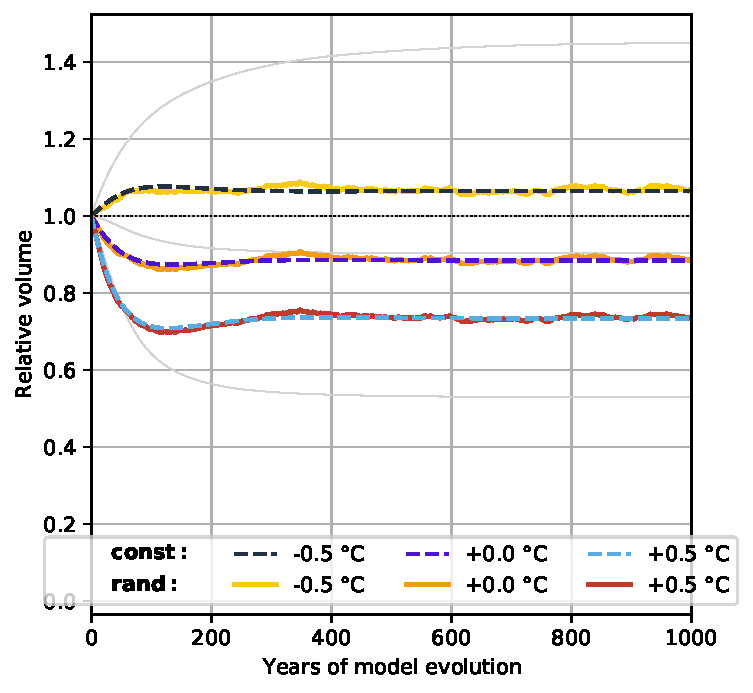
\includegraphics[width=\textwidth]{../plots/final_plots/time_series/histalp_commitment/volume_norm_vas.pdf}
      \end{subfigure}
      \hfill
      \begin{subfigure}[b]{0.48\textwidth}
        \caption{Flowline model, relative glacier volume}
        \label{fig:histalp_commitment:volume_norm_random}
        \centering
        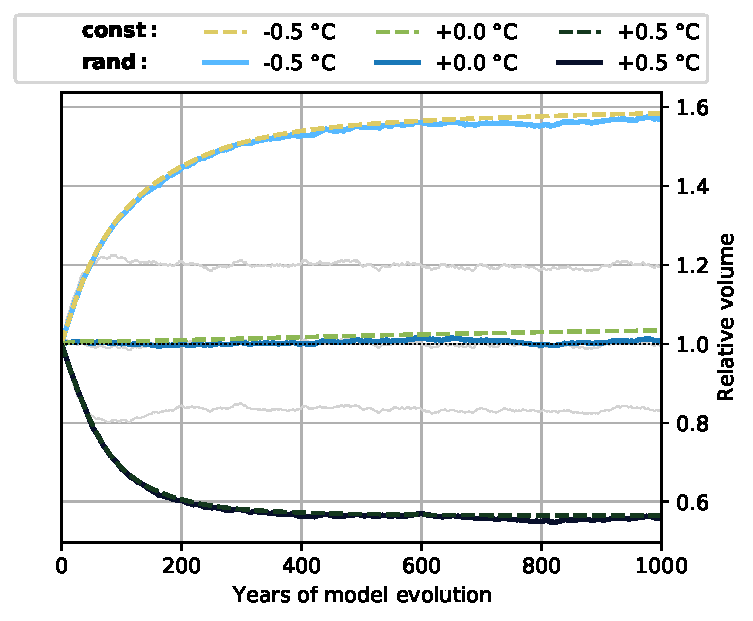
\includegraphics[width=\textwidth]{../plots/final_plots/time_series/histalp_commitment/volume_norm_fl.pdf}
      \end{subfigure}
      \begin{subfigure}[b]{0.48\textwidth}
        \caption{\Vas{} model, absolute glacier volume}
        \label{fig:histalp_commitment:volume_abs_const}
        \centering
        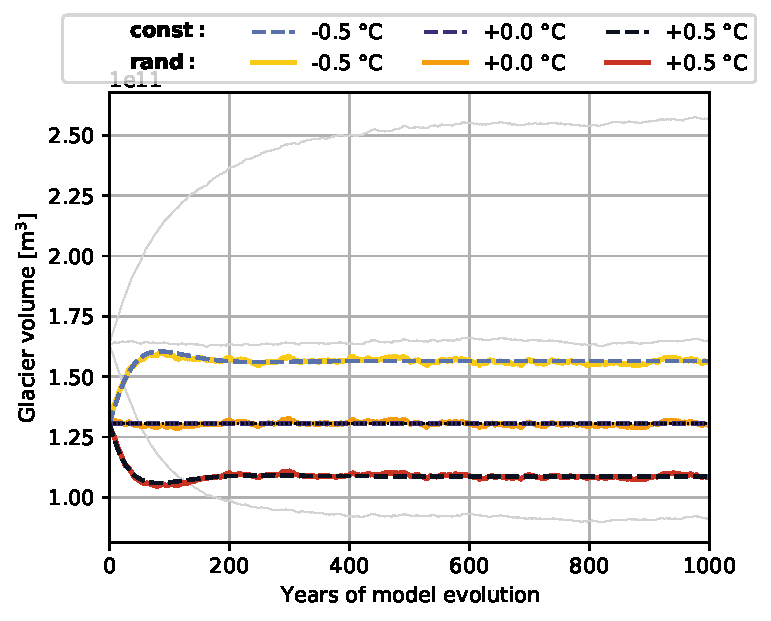
\includegraphics[width=\textwidth]{../plots/final_plots/time_series/histalp_commitment/volume_abs_vas.pdf}
      \end{subfigure}
      \hfill
      \begin{subfigure}[b]{0.48\textwidth}
        \caption{Flowline model, absolute glacier volume}
        \label{fig:histalp_commitment:volume_abs_random}
        \centering
        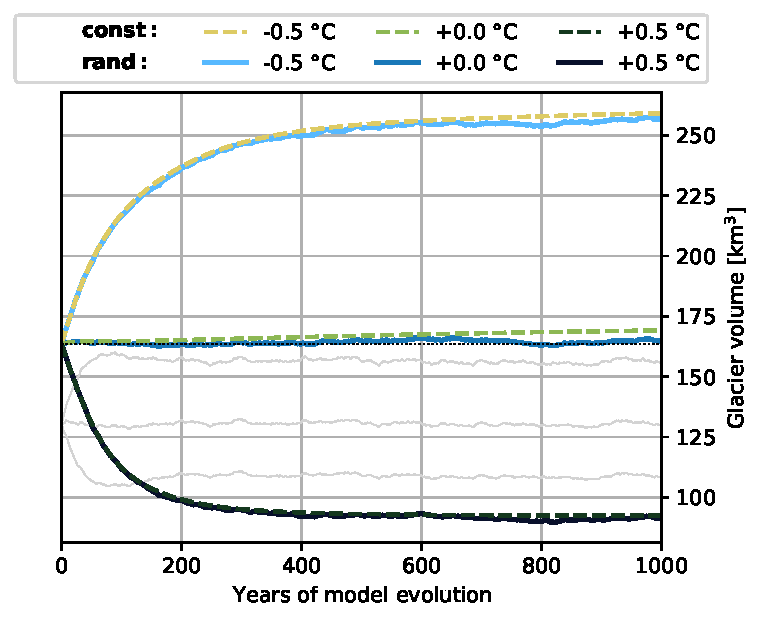
\includegraphics[width=\textwidth]{../plots/final_plots/time_series/histalp_commitment/volume_abs_fl.pdf}
      \end{subfigure}
      
      \caption{Time series of total ice volume for all glaciers in the HISTALP domain. The upper two panels show the relative glacier ice volume, normalized with the initial values, while the lower two panels show the absolute glacier ice volume. The left panels show the result of the \vas{} model, the right panels show the results of the flowline model. Solid lines represent the random climate scenarios, while dashed lines represent the constant climate scenarios. All climate scenarios are based on an equilibrium climate, with one of three different temperature biases.
      Yellow, orange and red solid lines represent the \vas{} model, while cyan, blue and purple solid lines represent the flowline model, under a random climate with a temperature bias of \SI{-.5}{\celsius}, \SI{0}{\celsius} and \SI{+.5}{\celsius}, respectively. Yellow, orange and red dashed lines represent the \vas{} model, while cyan, blue and purple dashed lines represent the flowline model, under a constant climate with a temperature bias of \SI{-.5}{\celsius}, \SI{0}{\celsius} and \SI{+.5}{\celsius}, respectively. %TODO change colors
      The dotted line indicate the initial volume. The light gray lines represent the volume evolutions of the other model, to facilitate comparisons.}
      \label{fig:histalp_commitment}
    \end{figure}

  % section regional_runs_with_all_alpine_glaciers_results (end)

  \section{Sensitivity experiments} % (fold)
  \label{sec:sensitivity_experiments_results}

    All the experiments performed above show quite large differences in projected ice volume change between the \vas{} model and the flowline model. However, the ``out-of-the-box'' scaling model is maybe not the best fit for the Alpine glaciers, and it is definitely not a good fit for any single glacier. Hence, tuning a set of parameters may improve the model performance.
    The most obvious tuning parameters are the model-internal time scales, and the scaling constants and scaling exponents. The following sensitivity experiments run the \vas{} model with different values for these parameters. As before, the experiments are performed on the Hintereisferner (RGI60-11.00897) and on all Alpine glaciers in the HISTALP domain, in each case with a constant equilibrium climate scenario and a positive temperature bias of \SI{+0.5}{\celsius}. For details about the experimental setup see Section~\ref{sub:sensitivity_experiments_setup}.

    \begin{tldrbox}[Sensitivity experiments]{tldr:sensitivity_experiments_results}
      \item The model-internal time scales control the damping ratio of the oscillation, longer time scales correspond to stronger overshoots.
      \item Halving the model-internal time scales leads to an almost asymptotic change in aggregate ice volume of the HISTALP domain, showing only negligible oscillations.
      \item Different scaling constants lead to a different initial ice volume and a different initial glacier length, which in turn affect the e-folding time scales.
      \item Changing the scaling constants has little to no effect on the normalized volume change and normalized equilibrium volume.
      \item Custom scaling constants and exponents increase the change in ice volume ever so slightly, but the results are still not comparable to the flowline model.
    \end{tldrbox}
    
    \begin{figure}[ht]
      \centering
      % HEF time scales
      \begin{subfigure}[b]{0.476\textwidth}
        \caption{Hintereisferner, different model-internal time scales}
        \label{fig:sensitivity:time_scales_hef}
        \centering
        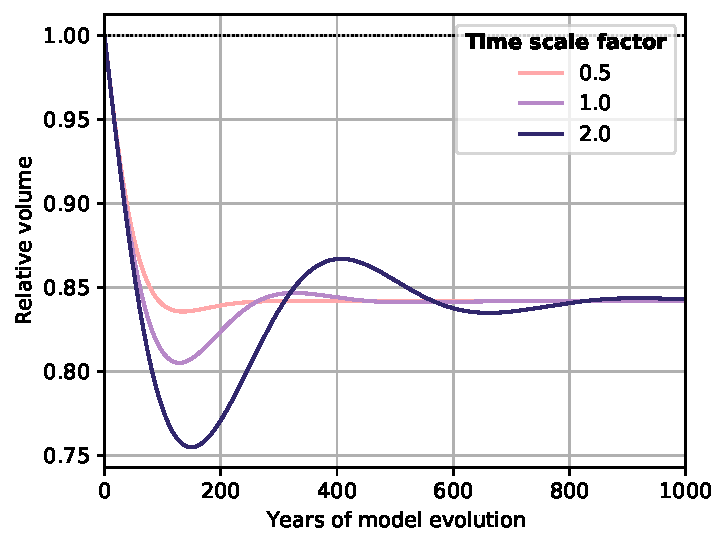
\includegraphics[width=\textwidth]{../plots/final_plots/sensitivity/time_scales_hef.pdf}
      \end{subfigure}
      \hfill
      % HEF scaling params
      \begin{subfigure}[b]{0.476\textwidth}
        \caption{Hintereisferner, different scaling constants}
        \label{fig:sensitivity:scaling_params_hef}
        \centering
        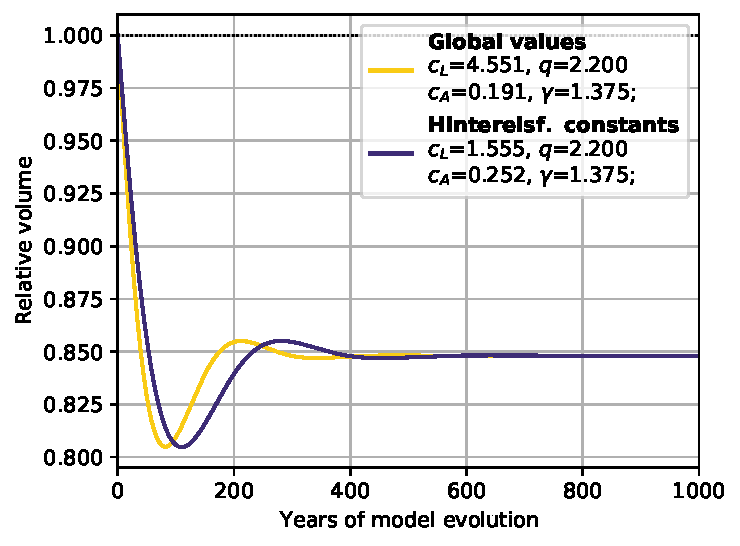
\includegraphics[width=\textwidth]{../plots/final_plots/sensitivity/scaling_params_hef.pdf}
      \end{subfigure}
      
      % HISTALP time scales
      \begin{subfigure}[b]{0.476\textwidth}
        \caption{HISTALP domain, different model-internal time scales}
        \label{fig:sensitivity:time_scales_histalp}
        \centering
        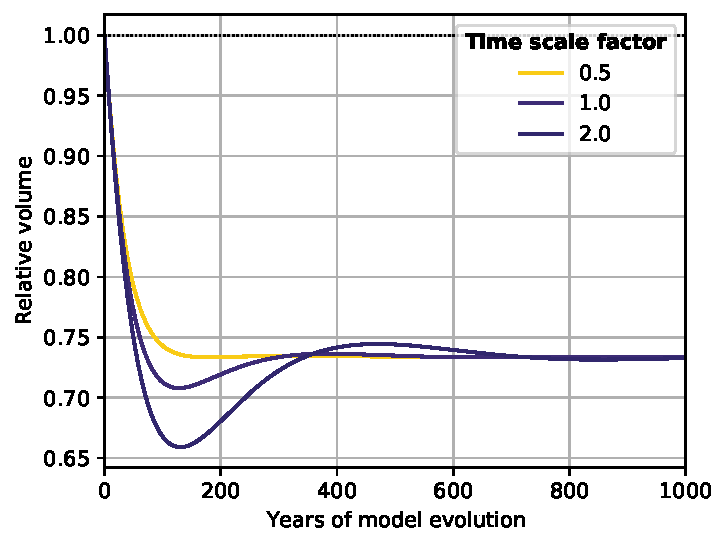
\includegraphics[width=\textwidth]{../plots/final_plots/sensitivity/time_scales_histalp.pdf}
      \end{subfigure}
      \hfill
      % HISTALP scaling params
      \begin{subfigure}[b]{0.476\textwidth}
        \caption{HISTALP domain, different scaling constants and scaling exponents}
        \label{fig:sensitivity:scaling_params_histalp}
        \centering
        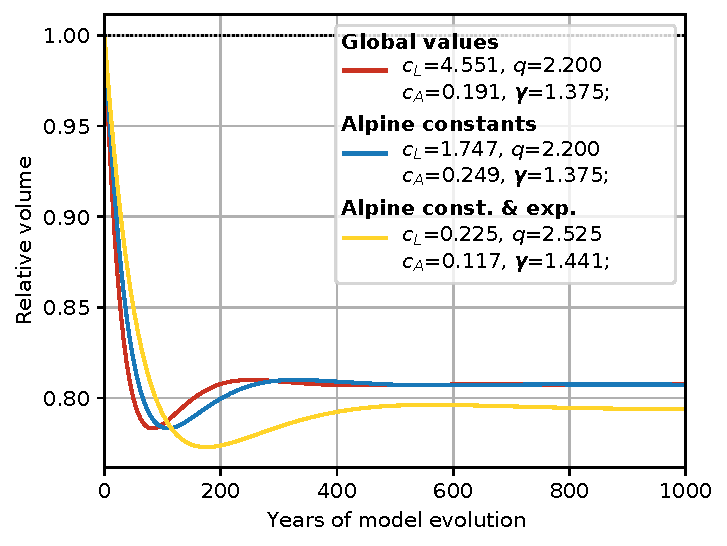
\includegraphics[width=\textwidth]{../plots/final_plots/sensitivity/scaling_params_histalp.pdf}
      \end{subfigure}
      
      \caption{Temporal evolution of glacier ice volume under a positive temperature bias of \SI{+0.5}{\celsius} for the Hintereisferner (RGI60-11.00897) in the two upper panels (\subref{fig:sensitivity:time_scales_hef}) and (\subref{fig:sensitivity:scaling_params_hef}) and for the entire HISTALP domain in the two lower panels (\subref{fig:sensitivity:time_scales_histalp}) and (\subref{fig:sensitivity:scaling_params_histalp}). The right panels show results for different model-internal time scales, scaled by a linear factor (see legend for details). The left panels show results for different scaling constants and scaling exponents (see legend for details). Note the difference in y-axis scales.}
      \label{fig:sensitivity}
    \end{figure}

    \subsection{Sensitivity to model-internal time scales} % (fold)
    \label{sec:sensitivity_to_model_internal_time_scales_results}
      Let's again start with the Hintereisferner test case, before moving to the regional scale. As was to be expected, the model-internal time scales do not affect the absolute values, but control only the oscillatory behavior. The e-folding response time scales for length and area are directly proportional to the model-internal time scales. Halving and doubling the time scales results in a respective change of \SI{-4}{\year} and \SI{+7}{\year} for the area response time and \SI{-10}{\year} and \SI{+15}{\year} for the length response time\footnote{The changes refer to the values shown in Section~\ref{sec:single_glacier_test_case_results}.}. The asymmetric responses hint at the non-linear effect of the time scales. Interestingly enough, the e-folding response time for volume is indirectly proportional to the model internal time scales, and changes only by \SI{\pm1}{\year}. This means, while the glacier takes longer to reach it's new equilibrium area and length, it takes less time to reach the new equilibrium volume (and vice versa). This is, however, most likely just a mathematical artifact, which stems from the oscillatory behavior and is discussed in the following.

      The main change, however, is seen in the oscillation amplitude (Figure~\ref{fig:sensitivity:time_scales_hef}). The damping ratio seems to be controlled by the model-internal time scales. Higher model-internal time scales lead to stronger oscillations and vice versa. But even with halved model-internal time scales, the modeled volume adjustment still shows some oscillations. With the default values, the \vas{} model overshoots the volume change estimate by \SI{5}{\percent} of the final equilibrium value and it takes 371 years to reach an equilibrium. Hereby, an equilibrium state is (somewhat arbitrarily) defined as the range of \SI{\pm0.1}{\percent} of the equilibrium value at year 1000. Halving and doubling the model-internal time scales changes the overshoot to \SI{1}{\percent} and \SI{11}{\percent} of the equilibrium value, respectively. The time span until a new equilibrium is reached seems to be almost linearly dependent on the model-internal time scales. By halving and doubling the model-internal time scales it takes 150 years and 688 years for the model to reach a new steady state, respectively.

      The same qualitative findings are made for the regional run with all Alpiner glaciers (Figure~\ref{fig:sensitivity:time_scales_histalp}). The absolute values do not change for different model-internal time scales, only the oscillatory behavior does. While longer model-internal time scales result again in stronger overshoots, the oscillations seem generally more damped for the regional run. This is most likely a side effect of the summation over all Alpine glacier, whereby small scale oscillations can cancel each other out. The overshoots amount to \SI{0.2}{\percent}, \SI{3.0}{\percent} and \SI{8.0}{\percent} of the equilibrium value for a time scale factor of 0.5, 1 and 2, respectively. Thereby it takes 133 years, 335 years and 642 years to reach a new steady state. When halving the model-internal time scales, the aggregate volume evolution shows almost no more discernible oscillations and is basically of exponential (asymptotic) nature.

    % subsection sensitivity_to_model_internal_time_scales_results (end)

    \subsection{Sensitivity to scaling parameters} % (fold)
    \label{sec:sensitivity_to_scaling_parameters_results}

      As seen above, the model-internal time scale do not change the absolute values of any geometric glacier property. So what about the scaling parameters?! The following paragraph compares the model behavior between the custom Hintereisferner scaling constants and the global scaling constants (Figure\ref{fig:sensitivity:scaling_params_hef}). The scaling exponents are held constant, since it is not possible to compute a linear regression from a single data point (see Section~\ref{sub:sensitivity_experiments_setup} for details). % $c_L = \SI{1.555}{\meter^{3-q}}$ and $c_A = \SI{0.252}{\meter^{3-2\gamma}}$ and the global scaling constants $c_L = \SI{4.551}{\meter^{3-q}}$ and $c_A = \SI{0.191}{\meter^{3-2\gamma}}$.
      Changing the scaling constants leads to different absolute values. As explained in Section~\ref{sub:glacier_evolution_model_implementation}, the \vas{} model starts by computing the initial glacier volume from the surface area via the \vas{} relation. Hence, the initial area stays the same while the initial ice volume increases with the custom scaling constants. The initial volume for the Hintereisferner increases to \SI{0.787}{\cubic\kilo\meter} with custom scaling constants $c_L = \SI{1.555}{\meter^{3-q}}$ and $c_A = \SI{0.252}{\meter^{3-2\gamma}}$, compared to the \SI{0.596}{\cubic\kilo\meter} with the global values. While starting with a larger initial ice volume increases the absolute change in ice volume (\SI{-0.120}{\cubic\kilo\meter} vs. \SI{-0.091}{\cubic\kilo\meter}), it still results in a larger equilibrium ice volume (\SI{0.667}{\cubic\kilo\meter} vs. \SI{0.506}{\cubic\kilo\meter}). However, when normalized with the respective initial ice volumes, the changes in ice volume, the equilibrium values and the overshoots (i.e., minimum values due to the oscillatory behavior) are almost identical (the differences lie far below \SI{0.1}{\percent}). This comes as no surprise, since the scaling constants are canceled out during the normalization process. In fact, when estimating \emph{changes} in regional or global ice volume the scaling constant $c$ can be eliminated altogether \citep[][Section 8.5]{Bahr2015}. While the relative values do not change, the temporal evolution does. As already discussed, the bigger custom scaling constant $c_A$ leads to a bigger initial ice volume. Increasing the glacier's ice volume in turn increases the glacier's response time, since larger glaciers generally react slower to climatic changes. The volume e-folding response time increases to 30 years with the custom scaling constants, compared to 23 years with the global values. The increased response time goes hand in hand with a stronger oscillation. While the amplitude stays the same, the frequency decreases. Hence, the peak of the overshoot shifts by 28 years (to year 100 after the initial climate perturbation) and it takes much longer to reach the new equilibrium state (493 years vs. 371 years).
      While the glacier length reacts analogously to the custom scaling constants, the surface area does not. This was to be expected, since the initial surface area does not depend on the scaling parameters. While the equilibrium value and the e-folding response time are practically not affected, the oscillation amplifies. In addition to the decreased frequency, as for ice volume and glacier length, the surface area overshoots by \SI{15\,761}{\square\meter} more under the custom scaling constants (which corresponds to \SI{\approx0.2}{\percent} of the equilibrium value).
      
      Again, the results of regional Alpine run (Figure\ref{fig:sensitivity:scaling_params_histalp}) are analogous to the Hintereisferner test case. While the Hintereisferner test case compares only the global and custom scaling constants, an additional run with custom scaling constants and scaling exponents is investigated (see Section~\ref{sub:sensitivity_experiments_setup} for details). As seen above, changing the scaling constants results in different absolute values (for the initial volume as well as for the final equilibrium volume). However, when normalized with the initial values only the run with custom scaling exponents shows a different (bigger) change in ice volume. The total modeled glacier ice volume shrinks from an initial \SI{229.7}{\cubic\kilo\meter} to a final \SI{182.4}{\cubic\kilo\meter}, subjected to a positive temperature bias of \SI{+0.5}{\celsius}. The change of \SI{-47.3}{\cubic\kilo\meter} corresponds to \SI{-21}{\percent} of the initial value. However, the result does still not compare to the \SI{-47}{\percent} of the flowline model and is not even significantly different from the \SI{-19}{\percent} for the other two \vas{} runs.

    % subsection sensitivity_to_scaling_parameters_results (end)


  % section sensitivity_experiments_results (end)

  \section{Commitment runs} % (fold)
  \label{sec:commitment_runs_results}

    The easiest way of projecting future glacier mass change is by so called commitment experiments. While an accurate projection should be forced by GCM ensemble data, based on different emission scenarios, a simpler approach will suffice for this qualitative comparison of the \vas{} and flowline model. Thereby, different possible warming scenarios can be simulated by committing to todays climate and adding different positive temperature biases. For details about the experimental setup see Section~\ref{sub:commitment_runs_setup}. Figure~\ref{fig:histalp_commitment} shows the evolution of relative and absolute ice volume of all Alpine glaciers under different warming scenarios.

    Before starting with the results, a disclaimer is in order. As can be seen in the sections above, the \vas{} has some flaws when compared to the flowline model. However, since no validation against observational data was performed, no statement about the accuracy of the model accuracy can be made here. All that said, the following section should be seen as the culmination of all the work done above. And while the results may not hold up or even be entirely meaningless compared to recently published projections, they can serve as reference point on what to expect from a flowline model compared to the \vas{} model.

    Again, all characteristic established for the \vas{} model can be seen here as well: initial ice volume and ice volume changes are underestimated; the new equilibrium values are reached faster; the ice volume estimations overshoot and rebound; the symmetric behavior can not be asses since only positive temperature perturbations are used. Expressed in numbers: the \vas{} model estimates an ice volume change of \SI{42}{\cubic\kilo\meter} and \SI{88}{\cubic\kilo\meter} from an initial \SI{130}{\cubic\kilo\meter} to a final \SI{88}{\cubic\kilo\meter} and \SI{42}{\cubic\kilo\meter} for todays climate with \SI{0}{\celsius} and \SI{+2}{\celsius}, respectively. This corresponds to a relative loss in ice volume of \SI{-68}{\percent} under the \SI{+2}{\celsius} warming scenario. The flowline model already estimates a relative ice loss \SI{-66}{\percent} for todays climate without any temperature bias. And after one-hundred years under the \SI{+2}{\celsius} warming scenario, only \SI{8}{\percent} of glacier ice are left. These differences are even more drastic in absolute numbers, since the flowline starts with \SI{34}{\cubic\kilo\meter} more total ice volume. This suggests that ice change projections made with scaling models are most likely lower bound estimates.

    \begin{figure}[htp]
      \centering
      \begin{subfigure}[b]{0.48\textwidth}
        \caption{\Vas{} model, relative glacier volume}
        \label{fig:histalp_projection:volume_norm_const}
        \centering
        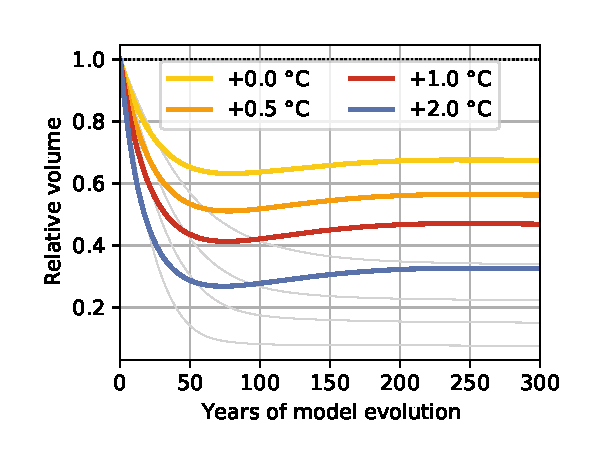
\includegraphics[width=\textwidth]{../plots/final_plots/time_series/histalp_projection/volume_norm_vas.pdf}
      \end{subfigure}
      \hfill
      \begin{subfigure}[b]{0.48\textwidth}
        \caption{Flowline model, relative glacier volume}
        \label{fig:histalp_projection:volume_norm_random}
        \centering
        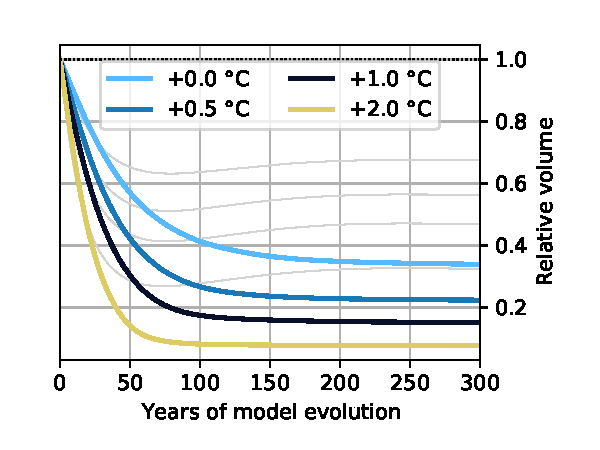
\includegraphics[width=\textwidth]{../plots/final_plots/time_series/histalp_projection/volume_norm_fl.pdf}
      \end{subfigure}
      \begin{subfigure}[b]{0.48\textwidth}
        \caption{\Vas{} model, absolute glacier volume}
        \label{fig:histalp_projection:volume_abs_const}
        \centering
        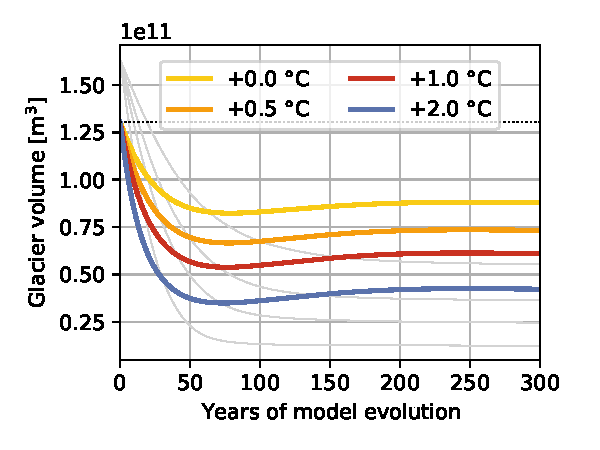
\includegraphics[width=\textwidth]{../plots/final_plots/time_series/histalp_projection/volume_abs_vas.pdf}
      \end{subfigure}
      \hfill
      \begin{subfigure}[b]{0.48\textwidth}
        \caption{Flowline model, absolute glacier volume}
        \label{fig:histalp_projection:volume_abs_random}
        \centering
        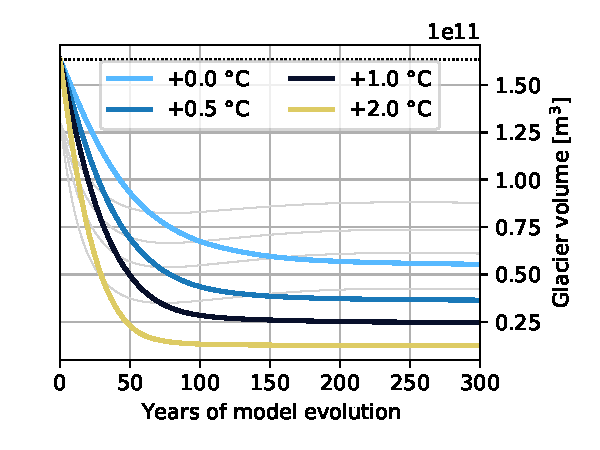
\includegraphics[width=\textwidth]{../plots/final_plots/time_series/histalp_projection/volume_abs_fl.pdf}
      \end{subfigure}
      
      \caption{Time series of total ice volume for all glaciers in the HISTALP domain. The upper two panels show the relative glacier ice volume, normalized with the initial values, while the lower two panels show the absolute glacier ice volume. The left panels show the result of the \vas{} model, the right panels show the results of the flowline model. Solid lines represent the random climate scenarios, while dashed lines represent the constant climate scenarios. All climate scenarios are based on an equilibrium climate, with one of three different temperature biases.
      Yellow, orange and red solid lines represent the \vas{} model, while cyan, blue and purple solid lines represent the flowline model, under a random climate with a temperature bias of \SI{-.5}{\celsius}, \SI{0}{\celsius} and \SI{+.5}{\celsius}, respectively. Yellow, orange and red dashed lines represent the \vas{} model, while cyan, blue and purple dashed lines represent the flowline model, under a constant climate with a temperature bias of \SI{-.5}{\celsius}, \SI{0}{\celsius} and \SI{+.5}{\celsius}, respectively. %TODO change colors
      The dotted line indicate the initial volume. The light gray lines represent the volume evolutions of the other model, to facilitate comparisons.}
      \label{fig:histalp_projection}
    \end{figure}


  % section commitment_runs_results (end)

% section future_projection (end)




